\documentclass[11pt]{article}

% ---------- packages ----------
\usepackage[a4paper,margin=2.2cm]{geometry}
\usepackage{amsmath,amssymb,amsthm}
\usepackage{xcolor}
\usepackage{tikz}
\usetikzlibrary{arrows.meta,positioning,fit,backgrounds,calc,shapes.geometric,decorations.pathreplacing,matrix}
\usepackage[most]{tcolorbox}
\usepackage{listings}
\usepackage{enumitem}
\usepackage{booktabs}
\usepackage{fontawesome5}
\usepackage{pifont}
\usepackage{microtype}
% allow \texttt / \ttfamily runs to break across lines so long identifiers
% like unordered_map<Company,(buy,sell)> don't overflow the margin.
\usepackage[htt]{hyphenat}
\newcommand{\allowttbreak}{\spaceskip=\fontdimen2\font plus \fontdimen3\font minus \fontdimen4\font}
\usepackage{hyperref}
\hypersetup{colorlinks=true,linkcolor=NavyBlue,urlcolor=teal,citecolor=teal,
  bookmarks=true,bookmarksopen=true,bookmarksopenlevel=1,
  pdftitle={The OrderCache Problem --- a playbook},pdfauthor={}}

% ---------- colors ----------
\definecolor{NavyBlue}{HTML}{1F3A93}
\definecolor{Accent}{HTML}{2E86DE}
\definecolor{Buy}{HTML}{27AE60}
\definecolor{Sell}{HTML}{C0392B}
\definecolor{Soft}{HTML}{F4F6F8}
\definecolor{Ink}{HTML}{22303C}
\definecolor{Gold}{HTML}{B8860B}
\definecolor{Codebg}{HTML}{F7F7FB}

% ---------- listings ----------
\lstdefinestyle{cpp}{
  language=C++, basicstyle=\ttfamily\small, keywordstyle=\color{NavyBlue}\bfseries,
  commentstyle=\color{gray!80}\itshape, stringstyle=\color{Sell},
  numbers=left, numberstyle=\tiny\color{gray}, numbersep=8pt,
  backgroundcolor=\color{Codebg}, frame=single, framesep=5pt, rulecolor=\color{gray!30},
  breaklines=true, showstringspaces=false, tabsize=2, columns=fullflexible,
  morekeywords={uint64_t,size_t,override,nullptr,constexpr,noexcept}
}
\lstset{style=cpp}

% ---------- theorem-ish boxes ----------
\newtcolorbox{keybox}[1][]{colback=Soft,colframe=Accent,boxrule=1pt,arc=3pt,
  left=8pt,right=8pt,top=6pt,bottom=6pt,title={#1},fonttitle=\bfseries\color{white},
  coltitle=white,colbacktitle=Accent}
\newtcolorbox{pitfall}[1][\faExclamationTriangle~Interview pitfall]{colback=red!4,colframe=Sell,
  boxrule=1pt,arc=3pt,left=8pt,right=8pt,top=6pt,bottom=6pt,title={#1},
  fonttitle=\bfseries\color{white},coltitle=white,colbacktitle=Sell}
\newtcolorbox{intu}[1][\faLightbulb~Intuition]{colback=Gold!8,colframe=Gold,
  boxrule=1pt,arc=3pt,left=8pt,right=8pt,top=6pt,bottom=6pt,title={#1},
  fonttitle=\bfseries\color{white},coltitle=white,colbacktitle=Gold}
\newtcolorbox{say}[1][\faComments~Say this out loud]{colback=Buy!6,colframe=Buy,
  boxrule=1pt,arc=3pt,left=8pt,right=8pt,top=6pt,bottom=6pt,title={#1},
  fonttitle=\bfseries\color{white},coltitle=white,colbacktitle=Buy}

\newcommand{\ty}[1]{\textsf{\textbf{#1}}}          % a type name
\newcommand{\code}[1]{\texttt{#1}}
\newcommand{\Buy}{\textcolor{Buy}{\textbf{Buy}}}
\newcommand{\Sell}{\textcolor{Sell}{\textbf{Sell}}}

\title{\vspace{-1.2cm}\Huge\bfseries The \textsf{OrderCache} Problem\\[4pt]
  \large\mdseries A type-driven, visual, from-scratch playbook\\
  \normalsize\itshape everything you need to internalize to nail the take-home}
\author{}
\date{}

\begin{document}
\maketitle
\vspace{-1.4cm}
\begin{center}\rule{0.9\linewidth}{0.6pt}\end{center}

\begin{abstract}\noindent
This document teaches the \textsf{OrderCache} take-home from the ground up. We will
(1) build the \emph{domain} in plain language, (2) model it with \emph{types}
(so the shape of the problem becomes obvious), (3) \emph{derive} the matching
formula from first principles and prove it is optimal, (4) pick \emph{data
structures} to make every operation fast, (5) walk through all six methods with
diagrams, and (6) hand you a one-page \emph{cheat sheet} of talking points and
gotchas. Read it once slowly; you will be able to reconstruct the whole solution
on a whiteboard from memory.
\end{abstract}

\tableofcontents
\clearpage

% ============ QUICK REFERENCE CARD (so you rarely need to flip) ============
\thispagestyle{empty}
\begin{tcolorbox}[colback=NavyBlue!4,colframe=NavyBlue,boxrule=1.2pt,arc=4pt,
  title={\bfseries Quick reference --- everything at a glance},fonttitle=\large\bfseries\color{white},coltitle=white,colbacktitle=NavyBlue]

\textbf{\color{NavyBlue}The matching formula} \hfill \emph{(hook + drills: \S6)}
\[
M=\min\!\Big(\underbrace{\textstyle\sum_c\min(b_c,\ S-s_c)}_{\text{each firm shops the market minus itself}},\ \ \underbrace{\min(B,S)}_{\text{never beat the smaller pile}}\Big)
\]
Equivalent (min-cut): $M=\min\big(B,\ S,\ B+S-\max_c(b_c+s_c)\big)$. \quad One firm $\Rightarrow 0$.

\medskip
\textbf{\color{NavyBlue}The four data structures} \hfill \emph{(derived: \S7)}
\begin{itemize}[leftmargin=1.3em,nosep]
  \item \code{orders\_}: \code{id$\to$Order} --- source of truth
  \item \code{ordersByUser\_}, \code{ordersBySecurity\_}: \code{key$\to$\{ids\}} --- indexes
  \item \code{securityTotals\_}: \code{secId$\to$\{B,\,S,\,per-company b/s\}} --- the aggregate
\end{itemize}

\medskip
\textbf{\color{NavyBlue}Complexity} \hfill \emph{(scorecard: \S7)}\\
add/cancel $O(1)$ \ $\vert$\ bulk cancels $O(k)$ \ $\vert$\ matching $O(\#\text{companies})$ \ $\vert$\ getAll $O(n)$

\medskip
\textbf{\color{NavyBlue}The gotchas that lose points} \hfill \emph{(full list: \S12)}\\
$\bullet$ not $\min(B,S)$ (company rule) \ $\bullet$ 64-bit sums \ $\bullet$ snapshot ids before bulk cancel \ $\bullet$ funnel writes through 2 helpers \ $\bullet$ graceful no-ops \ $\bullet$ \code{minQty} is \code{>=}

\medskip
\textbf{\color{NavyBlue}The four test layers} \hfill \emph{(thinking: \S8, drill: \S8)}\\
1.\ examples \ $\to$\ 2.\ edges (dominant company!) \ $\to$\ 3.\ relationships (add/cancel round-trip) \ $\to$\ 4.\ oracle + perf

\medskip
\hrule\smallskip
\footnotesize\emph{This PDF has clickable links and a bookmarks sidebar --- use your viewer's
outline panel to jump between sections instead of scrolling. Section numbers above
point you straight to the depth.}
\end{tcolorbox}
\clearpage

\section{The domain, from absolute scratch}

Forget code for a minute. A \textbf{financial exchange} is a place where people
say ``I want to buy 100 shares of X'' or ``I want to sell 500 shares of X''.
Each such statement is an \textbf{order}. Our job is to build the little
in-memory database (a ``cache'') that stores these orders and can answer one
interesting question quickly: \emph{how much trading can actually happen?}

\subsection{What is an order?}

An order is just six facts bundled together:

\begin{center}
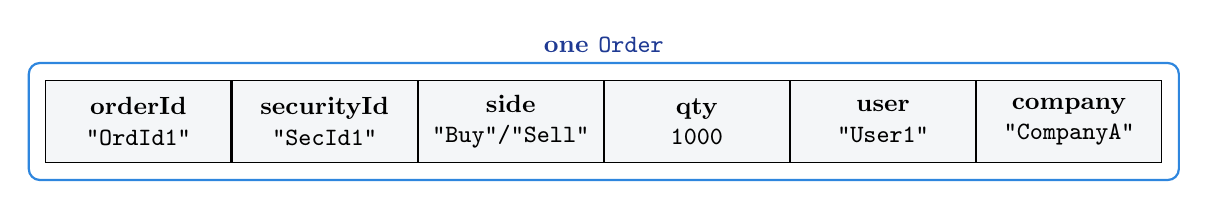
\begin{tikzpicture}[font=\small,node distance=0pt]
  \tikzstyle{cell}=[draw,minimum height=1.05cm,minimum width=2.35cm,align=center,fill=Soft]
  \node[cell] (id)   {\textbf{orderId}\\\ttfamily "OrdId1"};
  \node[cell,right=of id] (sec) {\textbf{securityId}\\\ttfamily "SecId1"};
  \node[cell,right=of sec] (side){\textbf{side}\\\ttfamily "Buy"/"Sell"};
  \node[cell,right=of side] (qty){\textbf{qty}\\\ttfamily 1000};
  \node[cell,right=of qty] (usr) {\textbf{user}\\\ttfamily "User1"};
  \node[cell,right=of usr] (co)  {\textbf{company}\\\ttfamily "CompanyA"};
  \begin{scope}[on background layer]
    \node[draw=Accent,thick,rounded corners,fit=(id)(co),inner sep=6pt,label=above:{\bfseries\color{NavyBlue}one \texttt{Order}}]{};
  \end{scope}
\end{tikzpicture}
\end{center}

\begin{itemize}[leftmargin=1.4em]
  \item \textbf{orderId} --- a unique name for \emph{this} order. Like a receipt number. No two orders share it.
  \item \textbf{securityId} --- \emph{what} is being traded (a stock, a bond\dots). Two orders ``match'' only if they are about the same security.
  \item \textbf{side} --- \Buy{} or \Sell. That is the only two possibilities.
  \item \textbf{qty} --- how many units. A positive whole number.
  \item \textbf{user} --- the person who placed the order.
  \item \textbf{company} --- which firm that person works for. \emph{This field is the twist of the whole problem}, as we will see.
\end{itemize}

\subsection{What does ``matching'' mean?}

Two orders can trade against each other --- \emph{match} --- when \textbf{all
three} of these hold:

\begin{center}
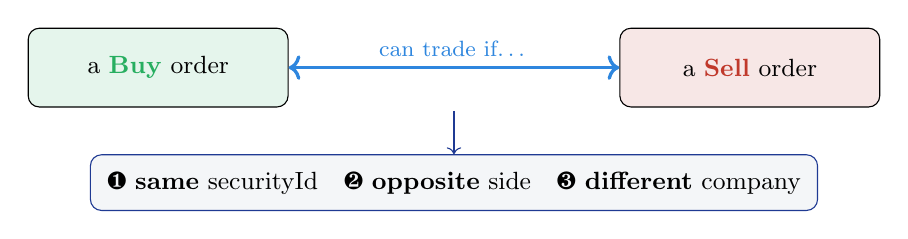
\begin{tikzpicture}[font=\small]
  \node[draw,fill=Buy!12,rounded corners,minimum width=3.3cm,minimum height=1cm,align=center] (b) {a \Buy{} order};
  \node[draw,fill=Sell!12,rounded corners,minimum width=3.3cm,minimum height=1cm,align=center,right=4.2cm of b] (s) {a \Sell{} order};
  \draw[<->,very thick,Accent] (b) -- node[above,align=center,font=\footnotesize]{can trade if\dots} (s);
  \node[below=1.1cm of $(b)!0.5!(s)$,align=center,draw=NavyBlue,rounded corners,fill=Soft,inner sep=6pt] (rule)
    {\ding{182}~\textbf{same} securityId\quad\ding{183}~\textbf{opposite} side\quad\ding{184}~\textbf{different} company};
  \draw[->,NavyBlue] ($(b)!0.5!(s)+(0,-0.55)$) -- (rule.north);
\end{tikzpicture}
\end{center}

Rules \ding{182} and \ding{183} are obvious (you can only trade the same thing, and
a buy needs a sell). Rule \ding{184} is the interesting one: \textbf{a company is
not allowed to trade with itself}. If CompanyA has both a buy and a sell for the
same security, those two \emph{cannot} cancel each other out --- presumably
because that would be a sham trade inside one firm.

\begin{intu}
Think of it as a dinner party where you may only shake hands with people from a
\emph{different} household. Your own family members don't count, no matter how
many of them are in the room.
\end{intu}

\subsection{The one hard question: \texttt{getMatchingSizeForSecurity}}

Given all the orders for one security, \textbf{how many total units can be
matched?} Matching consumes quantity: if a buy of 300 meets a sell of 500, then
300 units trade and the sell has 200 left over to match against \emph{someone
else}. We want the grand total of units that find a partner.

\begin{keybox}[Worked micro-example]
One security. Three orders:\\[2pt]
\Buy{} 100 (CompanyA)\qquad \Sell{} 100 (CompanyA)\qquad \Sell{} 100 (CompanyB)\\[4pt]
The buy is from A. It \emph{cannot} use A's sell (same company!). It \emph{can}
use B's sell. So $100$ units match. The answer is \textbf{100}, not 200 --- even
though there are 100 buy and 200 sell units sitting there.
\end{keybox}

\subsection{The six operations we must support}

\begin{center}
\begin{tabular}{@{}ll@{}}
\toprule
\textbf{Method} & \textbf{Plain English} \\
\midrule
\code{addOrder(order)} & remember a new order \\
\code{cancelOrder(id)} & forget one order by its id \\
\code{cancelOrdersForUser(user)} & forget \emph{every} order a person placed \\
\code{cancelOrdersForSecIdWithMinimumQty(sec,\,q)} & forget orders of a security with \code{qty}\,$\ge q$ \\
\code{getMatchingSizeForSecurity(sec)} & the hard question above \\
\code{getAllOrders()} & dump everything we're holding \\
\bottomrule
\end{tabular}
\end{center}

\noindent The whole game is: pick storage so that \emph{all six} are fast, even
with a million orders. Everything that follows is in service of that.

\subsection{How this document is built (the roadmap)}

Every section builds on the last, always from scratch:

\begin{center}
\renewcommand{\arraystretch}{1.25}\footnotesize
\begin{tabular}{@{}rl@{}}
\toprule
\S & \textbf{builds} \\
\midrule
1 & the domain (you are here) \\
2 & the \emph{types} --- how thinking in types shapes the design \\
2\textonehalf & \emph{math foundations from zero} --- sets, sums, optimization, graphs, flow, duality \\
3 & the matching \emph{formula}, discovered by hand then generalized \\
4 & the full \emph{mathematics} (flows, cuts, inclusion--exclusion) --- optional depth \\
4\textonehalf & \emph{LP duality} --- \emph{why} a min equals the max (the deepest ``why'') \\
5 & the \emph{design}, derived from a plain vector up to the four structures \\
6 & the six \emph{operations}, each derived from what it is handed \\
7 & the real \emph{implementation}, taught line by line (verified, compiles) \\
8--9 & \emph{testing} --- how to \emph{think} about tests, the theory, then real GoogleTest code \\
10 & a one-page \emph{cheat sheet} to rehearse from \\
\bottomrule
\end{tabular}
\end{center}

\noindent Read it once slowly and you can reconstruct the entire solution --- code
and tests --- on a whiteboard from understanding, not memory.

\clearpage
\section{Modeling with types (the type-driven lens)}

Here is the core idea in one sentence: \textbf{a type is the set of all values
something can possibly be}, and if we describe each piece of the problem by its
type, the correct data structures and algorithms almost fall out for free.

\begin{keybox}[A note on honesty --- ``type-driven'', not ``type theory'']
What follows is \emph{type-driven design} (the practical school: strong types,
enums, \code{std::optional}, ``make illegal states unrepresentable''). It is
\emph{not} formal type theory (Curry--Howard, dependent/refinement types, proofs).
That distinction matters: in a systems take-home the pragmatic version is exactly
right, and over-claiming ``type-theoretic'' to a reviewer who knows the difference
is a needless risk. Use the vocabulary below to \emph{reason}, then implement in
plain C++17. The three ways to build types --- and this problem uses all three:
\end{keybox}

\subsection{The three atoms}

\begin{center}
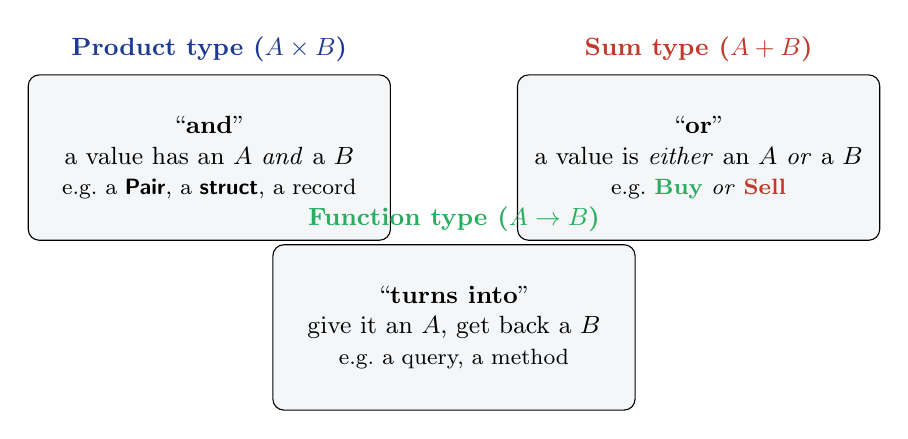
\begin{tikzpicture}[font=\small,every node/.style={align=center}]
  % product
  \node[draw,rounded corners,fill=Soft,minimum width=4.6cm,minimum height=2.1cm] (p) {};
  \node[above=1pt of p.north] {\bfseries\color{NavyBlue}Product type ($A\times B$)};
  \node at (p) {``\textbf{and}''\\a value has an $A$ \emph{and} a $B$\\\footnotesize e.g.\ a \ty{Pair}, a \ty{struct}, a record};
  % sum
  \node[draw,rounded corners,fill=Soft,minimum width=4.6cm,minimum height=2.1cm,right=1.6cm of p] (s) {};
  \node[above=1pt of s.north] {\bfseries\color{Sell}Sum type ($A+B$)};
  \node at (s) {``\textbf{or}''\\a value is \emph{either} an $A$ \emph{or} a $B$\\\footnotesize e.g.\ \Buy{} \emph{or} \Sell};
  % function
  \node[draw,rounded corners,fill=Soft,minimum width=4.6cm,minimum height=2.1cm,below=1.1cm of $(p)!0.5!(s)$] (f) {};
  \node[above=1pt of f.north] {\bfseries\color{Buy}Function type ($A\to B$)};
  \node at (f) {``\textbf{turns into}''\\give it an $A$, get back a $B$\\\footnotesize e.g.\ a query, a method};
\end{tikzpicture}
\end{center}

\begin{intu}
Why the names \emph{product} and \emph{sum}? Count the values! If $A$ has 3
possible values and $B$ has 4, then a pair $A\times B$ has $3\times4=12$
possibilities (a product), while a choice $A+B$ has $3+4=7$ (a sum). The
arithmetic is literally why they're named that. This ``counting values'' habit
is the single most useful trick type theory gives an interviewer.
\end{intu}

\subsection{Typing the \texttt{Order}}

An \code{Order} is a \textbf{product type} --- it bundles several fields with
``and''. In type-theory notation:
\[
\ty{Order} \;=\; \ty{OrderId}\;\times\;\ty{SecId}\;\times\;\ty{Side}\;\times\;\ty{Qty}\;\times\;\ty{User}\;\times\;\ty{Company}
\]
and \ty{Side} is a \textbf{sum type} with exactly two inhabitants:
\[
\ty{Side} \;=\; \Buy \;+\; \Sell.
\]

\begin{pitfall}
The starter code stores \code{side} as a \code{std::string}. Type-theoretically
that is \emph{wrong}: a string has billions of possible values (\code{"Buy"},
\code{"buy"}, \code{"BUY"}, \code{"xyz"}\dots), but \ty{Side} has only
\textbf{two}. The gap between ``what the type allows'' and ``what is actually
valid'' is exactly where bugs live. In the interview, \emph{say} you would
normalize it to a 2-value \code{enum} internally (\code{Buy}/\code{Sell}) --- that
turns a whole class of invalid states into \emph{unrepresentable} states. This is
the famous principle: \emph{make illegal states unrepresentable}.
\end{pitfall}

\subsection{Typing the operations --- their signatures tell you the plan}

Read each method as a function type. The \emph{shape} of the arrow tells you what
data structure you need to make it fast.

\begin{center}
\renewcommand{\arraystretch}{1.5}
\begin{tabular}{@{}p{5.9cm}p{8.3cm}@{}}
\toprule
\textbf{Type signature} & \textbf{What the shape demands} \\
\midrule
$\code{add}:\ \ty{Order}\to\ty{Unit}$ &
returns nothing (\ty{Unit} = the 1-value type, ``void''); it's a \emph{mutation}. Must update every index. \\
$\code{cancel}:\ \ty{OrderId}\to\ty{Unit}$ &
we're handed only an \emph{id}. So we need a map \ty{OrderId}$\to$\ty{Order} to find the rest. \\
$\code{cancelForUser}:\ \ty{User}\to\ty{Unit}$ &
handed a \emph{user}. So we need \ty{User}$\to$\ty{Set of OrderId} to avoid scanning everything. \\
$\code{cancelForSecMinQty}:\ \ty{SecId}\times\ty{Qty}\to\ty{Unit}$ &
handed a \emph{security}. So we need \ty{SecId}$\to$\ty{Set of OrderId} too. \\
$\code{matchSize}:\ \ty{SecId}\to\ty{Qty}$ &
the money method: a \ty{SecId} in, a single number out. This is a \emph{fold} (aggregate) --- see \S3. \\
$\code{getAll}:\ \ty{Unit}\to\ty{List}\,\ty{Order}$ &
dump: needs a way to enumerate every live order. \\
\bottomrule
\end{tabular}
\end{center}

\begin{keybox}[The punchline of this section]
Every method that takes a key of type \ty{K} and must act on all orders with that
key is screaming for a map \ty{K}$\to$\ty{Set of OrderId}. Three different keys
(\ty{OrderId}, \ty{User}, \ty{SecId}) appear as inputs, so we will keep
\textbf{three indexes}. \emph{The type signatures alone told us how many indexes
to build.}
\end{keybox}

\subsection{The cache itself as a type}

The whole cache is a product of one \emph{source of truth} plus several
\emph{derived indexes} plus \emph{pre-computed aggregates}:
\[
\ty{OrderCache} \;=\;
\underbrace{(\ty{OrderId}\!\to\!\ty{Order})}_{\text{truth}}\;\times\;
\underbrace{(\ty{User}\!\to\!\mathcal{P}\ty{OrderId})}_{\text{index}}\;\times\;
\underbrace{(\ty{SecId}\!\to\!\mathcal{P}\ty{OrderId})}_{\text{index}}\;\times\;
\underbrace{(\ty{SecId}\!\to\!\ty{Aggregate})}_{\text{pre-sum}}
\]
where $\mathcal{P}$ means ``powerset'' = ``a set of''. The last factor is the
clever one that makes \code{matchSize} fast; we derive its exact contents next.

\begin{say}
``I'd model \code{Order} as a product type and \code{Side} as a two-value sum,
normalizing the string to an enum so illegal sides are unrepresentable. Each
operation's signature is a function type, and the key it takes tells me which
index it needs --- that's why I keep one map from each of orderId, user, and
securityId. The matching query is a fold over a per-security aggregate I maintain
incrementally.''
\end{say}

\clearpage
\section{Mathematical foundations, from zero}

This section assumes you know \emph{nothing} and builds every mathematical idea the
rest of the document leans on --- sets, sums, functions, $\min/\max$, optimization,
bounds, counting, graphs, matching, and flow. Each idea is introduced in plain
language, with a picture, and then connected to the \textsf{OrderCache} problem so
you see \emph{why} it's here. Read it once and the ``mathy'' sections will feel
obvious.

\subsection{Numbers, and the only two operations we really need}

Almost everything here is built from two humble operations on whole numbers:

\begin{itemize}[leftmargin=1.5em]
  \item $\min(a,b)$ --- the \textbf{smaller} of two numbers. $\min(3,7)=3$.
  \item $\max(a,b)$ --- the \textbf{larger}. $\max(3,7)=7$.
\end{itemize}

They generalize to many arguments: $\min(4,1,9,2)=1$. That's it. When you see a
scary formula later, it is almost always ``take the smaller/larger of a few
sensible quantities''. $\min$ shows up whenever something is \textbf{limited by its
tightest constraint} (a chain is as strong as its weakest link); $\max$ whenever we
hunt for the \textbf{worst bottleneck}.

\subsection{Sets and multisets --- bags of things}

A \textbf{set} is a collection of distinct things, written in braces:
$\{A, B, C\}$. Order doesn't matter and duplicates don't count:
$\{A,A,B\}=\{A,B\}$.

A \textbf{multiset} (or ``bag'') is like a set but duplicates \emph{do} count:
the bag $[\![A,A,B]\!]$ has two $A$'s. Our orders are really a \textbf{bag}: two
different orders can be identical in every field except their id.

\begin{intu}
Why care? Because the matching answer depends only on the \emph{bag} of orders,
not the order you inserted them. That single fact is why ``insertion order doesn't
change the answer'' is a law we can test (\S on testing). Recognizing something as
a set vs.\ a bag tells you what may and may not matter.
\end{intu}

\subsection{Functions --- machines that turn an input into an output}

A \textbf{function} is a rule: give it an input, get exactly one output. We write
$f : X \to Y$ to mean ``$f$ takes an $X$ and returns a $Y$''. The arrow is the
whole idea: \emph{in-type} on the left, \emph{out-type} on the right.

\begin{center}
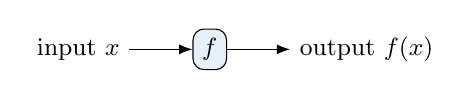
\begin{tikzpicture}[font=\small,>=Latex]
  \node (x) {input $x$};
  \node[draw,rounded corners,fill=Accent!12,right=8mm of x] (f) {$f$};
  \node[right=8mm of f] (y) {output $f(x)$};
  \draw[->](x)--(f); \draw[->](f)--(y);
\end{tikzpicture}
\end{center}

Every operation in the cache is a function, and its arrow tells you its job:
\code{getMatchingSizeForSecurity} is $\ty{SecId}\to\ty{Number}$ --- one security in,
one number out. Because it turns a \emph{whole collection} (all the security's
orders) into \emph{one} number, it is a special kind of function called a
\textbf{fold} (or aggregate); we meet folds properly in the operations section.

\subsection{Sigma notation --- a compact way to say ``add these up''}

The symbol $\sum$ (Greek capital sigma, ``S'' for \emph{sum}) just means ``add up
a list''. Read
\[
\sum_{c} g(c)
\]
as: ``for each item $c$, compute $g(c)$, and add all those results together.''
For example, if the companies are $A,B,C$ and $g$ is ``that company's buys'', then
$\sum_c g(c) = g(A)+g(B)+g(C)$ = total buys.

\begin{intu}
$\sum$ is a \code{for}-loop with a running total, written in one symbol. When you
see $\sum_c \min(b_c, S - s_c)$ later, mentally unroll it: ``loop over companies,
add up each one's $\min(\dots)$.'' Nothing more.
\end{intu}

\subsection{Optimization --- ``the best you can do, subject to limits''}

An \textbf{optimization problem} has two parts:
\begin{enumerate}[leftmargin=1.6em,nosep]
  \item an \textbf{objective}: a number you want to make as big (or small) as
        possible --- e.g.\ ``total quantity matched'';
  \item \textbf{constraints}: rules you may not break --- e.g.\ ``no company
        trades more than it has'', ``no self-trading''.
\end{enumerate}
``Maximize the objective without breaking any constraint'' is the entire game.
Matching is exactly this: \emph{maximize matched quantity, subject to per-company
limits and the different-company rule.}

\subsection{Upper bounds --- proving you \emph{can't} do better}

A subtle but powerful idea. Suppose you've matched $150$ units and wonder: is that
the best possible, or could a cleverer arrangement do more? An \textbf{upper bound}
is a number you can \emph{prove} the answer never exceeds. If you find a matched
value that \emph{equals} an upper bound, you're done --- it's optimal, no cleverness
left to find.

\begin{center}
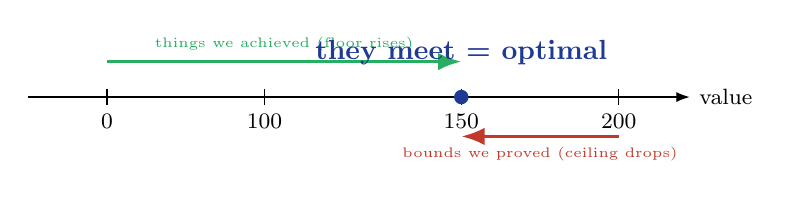
\begin{tikzpicture}[font=\footnotesize,>=Latex]
  \draw[->] (0,0) -- (8.4,0) node[right]{value};
  \foreach \x/\l in {1/0,3/100,5.5/150,7.5/200} \draw (\x,0.1)--(\x,-0.1) node[below]{\l};
  \draw[Buy,very thick,->] (1,0.45)--(5.5,0.45) node[midway,above,font=\tiny]{things we achieved (floor rises)};
  \draw[Sell,very thick,->] (7.5,-0.5)--(5.5,-0.5) node[midway,below,font=\tiny]{bounds we proved (ceiling drops)};
  \filldraw[NavyBlue] (5.5,0) circle (2.4pt) node[above=8pt,font=\bfseries]{they meet = optimal};
\end{tikzpicture}
\end{center}

\begin{intu}
Optimization is a squeeze: you push a \emph{floor} up (``I achieved this'') and a
\emph{ceiling} down (``you can't beat this''). When floor meets ceiling, that
number is the answer. This ``floor meets ceiling'' is the soul of \emph{duality},
which we reach shortly.
\end{intu}

\subsection{Counting and the bottleneck principle}

Two counting ideas power the whole matching result.

\textbf{The smaller-pile rule.} If you pair items from a red pile and a blue pile,
you can make at most $\min(\text{red},\text{blue})$ pairs --- the smaller pile runs
out first. This is why $\min(B,S)$ (total buy vs.\ total sell) is always a ceiling
on matching.

\textbf{Inclusion--exclusion.} To count a combined quantity without double-counting
or wrongly-counting, you \emph{include} everything, then \emph{exclude} the part
that shouldn't be there:
\[
\text{count} = (\text{everything}) - (\text{the forbidden part}).
\]
Concretely, if two overlapping groups have sizes $|X|$ and $|Y|$ and share $|X\cap
Y|$, the union is $|X|+|Y|-|X\cap Y|$ --- add both, subtract the overlap you
counted twice. In matching, the ``forbidden part'' we subtract is the quantity
trapped inside a single company (which may not trade with itself). That subtraction
is exactly the $-\,\max_c(b_c+s_c)$ you'll see in the closed form.

\subsection{Graphs --- dots and lines}

A \textbf{graph} is just \textbf{dots} (called \emph{nodes} or \emph{vertices})
connected by \textbf{lines} (\emph{edges}). That's the entire definition. Edges can
carry a number, a \textbf{capacity} (``at most this much may pass'').

A \textbf{bipartite} graph is one where the dots split into two teams, and edges
only go \emph{between} teams, never within. Buyers on the left, sellers on the
right, an edge for each allowed trade --- that's bipartite, and it's a picture of
our whole problem.

\begin{center}
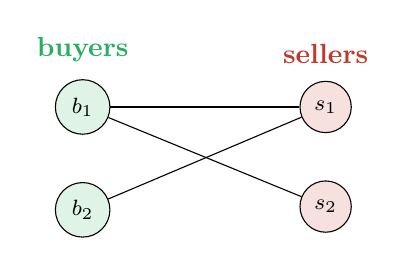
\begin{tikzpicture}[font=\footnotesize,>=Latex,node distance=6mm]
  \node[draw,circle,fill=Buy!15] (b1){$b_1$};
  \node[draw,circle,fill=Buy!15,below=of b1] (b2){$b_2$};
  \node[draw,circle,fill=Sell!15,right=2.4cm of b1] (s1){$s_1$};
  \node[draw,circle,fill=Sell!15,below=of s1] (s2){$s_2$};
  \draw (b1)--(s2); \draw (b2)--(s1); \draw (b1)--(s1);
  \node[above=1mm of b1,font=\bfseries\color{Buy}]{buyers};
  \node[above=1mm of s1,font=\bfseries\color{Sell}]{sellers};
\end{tikzpicture}
\end{center}

\subsection{Flow --- pushing stuff through a network}

Add a \textbf{source} (call it $s$, where stuff originates) and a \textbf{sink}
($t$, where it drains), and let quantity \emph{flow} along edges without ever
exceeding a capacity. The \textbf{max-flow} question is: \emph{what is the most we
can push from $s$ to $t$?}

\begin{center}
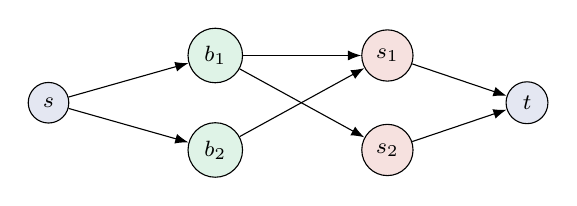
\begin{tikzpicture}[font=\footnotesize,>=Latex,node distance=7mm]
  \node[draw,circle,fill=NavyBlue!12] (s){$s$};
  \node[draw,circle,fill=Buy!15,right=1.5cm of s,yshift=6mm] (a){$b_1$};
  \node[draw,circle,fill=Buy!15,right=1.5cm of s,yshift=-6mm] (b){$b_2$};
  \node[draw,circle,fill=Sell!15,right=1.5cm of a] (c){$s_1$};
  \node[draw,circle,fill=Sell!15,right=1.5cm of b] (d){$s_2$};
  \node[draw,circle,fill=NavyBlue!12,right=1.5cm of $(c)!0.5!(d)$] (t){$t$};
  \draw[->](s)--(a);\draw[->](s)--(b);
  \draw[->](a)--(d);\draw[->](b)--(c);\draw[->](a)--(c);
  \draw[->](c)--(t);\draw[->](d)--(t);
\end{tikzpicture}
\end{center}

Matching \emph{is} a max-flow: push matched quantity from a source, through
buyers, across allowed (different-company) edges, into sellers, out to a sink.
The most you can push is the most you can match.

\subsection{Cuts, and the theorem that turns flow into a formula}

A \textbf{cut} is any way to slice the network into an $s$-side and a $t$-side; its
\textbf{cost} is the total capacity of edges pointing from the $s$-side to the
$t$-side --- a ``bottleneck.'' The celebrated \textbf{max-flow min-cut theorem}
says:
\[
\boxed{\ \text{maximum flow} \;=\; \text{minimum cut}\ .}
\]
The most you can push equals the \emph{cheapest} bottleneck. This is the bridge
from a hard ``arrange all the trades'' problem to an easy ``take the smallest of a
few numbers'' formula --- because finding the cheapest cut is just a $\min$.

\begin{intu}
Water pipes: the most water from tap to drain is capped by the narrowest section
of pipe the water must all squeeze through. ``Max-flow $=$ min-cut'' is the precise
version of that everyday fact. And ``min of a few bottlenecks'' is exactly the
shape of our closed-form answer.
\end{intu}

\subsection{Duality, in one paragraph}

The deepest idea, previewed here and expanded in its own section. Every ``maximize''
problem has a shadow ``minimize'' problem, and for these \emph{linear} problems the
two give the \emph{same number}. Maximizing matched quantity (hard, combinatorial)
equals minimizing over bottlenecks (easy, a $\min$). That equality is
\textbf{strong duality}, and ``max-flow $=$ min-cut'' is its most famous instance.
It's \emph{why} a minimum of three numbers can equal a maximum matching --- not an
approximation, an exact equality.

\subsection{The map --- how each idea lands on \textsf{OrderCache}}

\begin{center}
\renewcommand{\arraystretch}{1.3}\footnotesize
\begin{tabular}{@{}ll@{}}
\toprule
\textbf{Foundation} & \textbf{Where it shows up} \\
\midrule
$\min$ / smaller-pile rule & the $\min(B,S)$ cap on matching \\
$\max$ / worst bottleneck & the $\max_c(b_c+s_c)$ dominant-company term \\
bag (multiset), not set & why insertion order can't change the answer \\
function arrow $X\to Y$ & each method's signature; matching is $\ty{SecId}\to\ty{Number}$ \\
$\sum$ notation & the per-company reach $\sum_c\min(b_c,S-s_c)$ \\
optimization & ``maximize matched qty subject to the rules'' \\
upper bound / squeeze & why the formula is provably optimal, not a guess \\
inclusion--exclusion & subtracting the trapped, self-conflicted company \\
bipartite graph + flow & the model of buyers/sellers and legal trades \\
max-flow min-cut & turns the model into a closed-form $\min$ \\
duality & the reason that $\min$ equals the true maximum \\
\bottomrule
\end{tabular}
\end{center}

\noindent With these in hand, the next sections --- the formula, the full
mathematics, and LP duality --- are just these ideas applied to one concrete
problem.

\clearpage
\section{The matching formula, built from zero}

This is the section that wins the take-home. We build the formula the way you'd
actually discover it: start with a tiny example, match it \emph{by hand}, notice
the pattern, generalize, then prove it. No formula is dropped on you --- every
piece is earned.

\subsection{Step 1 --- the no-rules baseline}

Ignore the company rule for a moment. If any buy can meet any sell, matching is
trivial: pour the smaller side into the larger. With $B$ total buy and $S$ total
sell,
\[
M_{\text{naive}}=\min(B,S).
\]
You're limited by whichever side runs out first. Hold onto this --- it will come
back as a \emph{cap}, just not as the whole answer.

\subsection{Step 2 --- turn the rule on, watch the baseline break}

Now add the real rule: \Buy{} and \Sell{} match only across \textbf{different}
companies. Two tiny examples:

\begin{center}
\begin{tabular}{@{}p{6.6cm}p{6.6cm}@{}}
\textbf{Example X}\newline \Buy{}100(A),\ \Sell{}100(A),\ \Sell{}100(B) &
\textbf{Example Y}\newline \Buy{}100(A),\ \Sell{}100(A) \\[6pt]
$B{=}100,\ S{=}200 \Rightarrow M_{\text{naive}}{=}100$ &
$B{=}100,\ S{=}100 \Rightarrow M_{\text{naive}}{=}100$ \\[4pt]
\textcolor{Buy}{Correct: \textbf{100}} (A buys from B) &
\textcolor{Sell}{Correct: \textbf{0}} (A can't trade with itself!) \\
\end{tabular}
\end{center}

Example Y is the killer: naive says $100$, the truth is $0$. The baseline is
\emph{blind to who owns each unit}.

\begin{pitfall}
Saying ``it's just $\min$ of the two sides'' is the \#1 way people fail this. The
company rule forces you to reason \emph{per company}, not just per side.
\end{pitfall}

\subsection{Step 2\textonehalf --- picture what ``matching'' physically is}

Before the algebra, see it. A match is a \textbf{handshake} between one \Buy{} unit
and one \Sell{} unit from \emph{different} firms. Quantity is just ``how many
hands''. Here is Example X drawn out:

\begin{center}
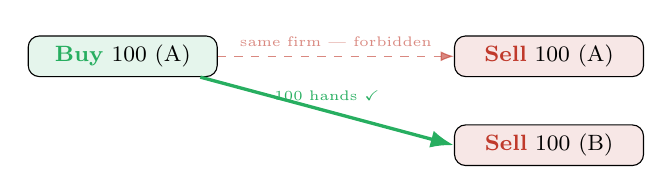
\begin{tikzpicture}[font=\footnotesize,>=Latex,node distance=5mm]
  \node[draw,rounded corners,fill=Buy!12,minimum width=2.4cm] (bA) {\Buy{} 100 (A)};
  \node[draw,rounded corners,fill=Sell!12,minimum width=2.4cm,right=3cm of bA] (sA) {\Sell{} 100 (A)};
  \node[draw,rounded corners,fill=Sell!12,minimum width=2.4cm,below=6mm of sA] (sB) {\Sell{} 100 (B)};
  \draw[->,very thick,Buy] (bA) -- node[above,font=\tiny]{100 hands \checkmark} (sB.west);
  \draw[->,dashed,Sell,opacity=.6] (bA) -- node[above,sloped,font=\tiny]{same firm --- forbidden} (sA);
\end{tikzpicture}
\end{center}

A's buy \emph{cannot} shake A's own sell (dashed, forbidden). It \emph{can} shake
B's sell. So $100$ units trade. The whole problem is: \emph{maximise the total
number of legal handshakes.}

\subsection{Step 3 --- match one example by hand, slowly}

Take a slightly bigger security and do the accounting a company at a time:
\[
\Buy{}100(A),\quad \Sell{}100(A),\quad \Sell{}100(B),\quad \Buy{}300(B).
\]
First tabulate per company --- just add up each firm's buys and sells:
\begin{center}
\begin{tabular}{@{}lll@{}}
\toprule
company & buys & sells \\
\midrule
A & $100$ & $100$ \\
B & $300$ & $100$ \\
\midrule
\textbf{total} & $B{=}400$ & $S{=}200$ \\
\bottomrule
\end{tabular}
\end{center}

Now the key question, asked \emph{once per buying company}: \textbf{``How much can
this firm actually buy?''} A firm is squeezed between two limits:
\begin{enumerate}[leftmargin=1.6em,nosep]
  \item how much it \emph{wants} to buy ($b_c$), and
  \item how much it is \emph{allowed} to buy from --- the sells belonging to
        \emph{other} firms.
\end{enumerate}
That second limit is the whole trick. Total sells in this security $=200$. But a
firm may not touch its \emph{own} sells, so the sells it may legally use are
\[
\underbrace{200}_{\text{all sells } S}\ -\ \underbrace{s_c}_{\text{its own sells}}.
\]
Work it firm by firm:
\begin{itemize}[leftmargin=1.4em]
  \item \textbf{Company A} wants $100$. Sells it may use $= 200 - \underbrace{100}_{s_A} = 100$.
        So A grabs $\min(\underbrace{100}_{\text{wants}}, \underbrace{100}_{\text{allowed}}) = \mathbf{100}$.
  \item \textbf{Company B} wants $300$. Sells it may use $= 200 - \underbrace{100}_{s_B} = 100$.
        So B grabs $\min(300, 100) = \mathbf{100}$.
\end{itemize}
Add the grabs: $100 + 100 = \mathbf{200}$. And the smaller pile is
$\min(B,S)=\min(400,200)=200$, so the cap doesn't bite. \textbf{Answer: 200}
(a true max-flow solver agrees). \emph{You just executed the formula without
knowing its name.}

\subsection{Step 4 --- name the pattern}

Look at what we did to each company $c$. Let $b_c,s_c$ be its buy/sell, $S$ the
security's total sell. The reach of company $c$ was
\[
\min\big(b_c,\ \underbrace{S-s_c}_{\text{sells $c$ may legally use}}\big).
\]
Summing over buying companies and capping by the smaller side (Step 1's baseline)
gives the whole thing:
\[
\boxed{\;M \;=\; \min\!\Big(\underbrace{\textstyle\sum_{c}\min\big(b_c,\;S-s_c\big)}_{\text{total per-company reach}},\ \ \min(B,S)\Big)\;}
\]

\begin{intu}
Read $S-s_c$ as ``the market minus yourself''. Each buying firm thinks: ``I want
$b_c$, but I may only shop from \emph{other} firms, who between them offer
$S-s_c$; so realistically I get the smaller of the two.'' Add up everyone's
realistic gets --- then the outer $\min(B,S)$ stops overlapping reaches from
claiming more trades than physically exist.
\end{intu}

\subsection{Step 5 --- sanity-check the two extremes}

\begin{itemize}[leftmargin=1.4em]
  \item \textbf{Example Y} (\Buy{}100(A), \Sell{}100(A)): only company A, and
        $S-s_A = 100-100 = 0$, so A's reach is $\min(100,0)=0$. Total $=\mathbf{0}$.
        \checkmark\ The formula \emph{knows} a firm can't trade with itself.
  \item \textbf{No company rule at all} (imagine every order a different firm):
        then $s_c=0$ for each buyer, reach $=\min(b_c,S)$, and the sum capped by
        $\min(B,S)$ collapses to $\min(B,S)$ --- the Step 1 baseline. \checkmark\
        The formula \emph{contains} the naive answer as a special case.
\end{itemize}

\subsection{Step 6 --- why not just simulate greedily?}

Tempting: walk the buys, and for each, eat sells in order, skipping same-company.
\textbf{That is wrong.} Greedy first-come matching can strand quantity a smarter
pairing would have used --- in fuzz testing it under-counted on thousands of
cases. The closed form is the provable optimum, so use it. (\S4 shows \emph{why}:
optimal matching needs flow-style re-routing, which greedy lacks.)

\subsection{Step 7 --- is it \emph{provably} right?}

Two independent checks while developing this:
\begin{enumerate}[leftmargin=1.4em]
  \item Reproduces all three problem-statement examples exactly (the $2700$ case
        and the full Example~2 / Example~3 tables).
  \item Matched a \textbf{true max-flow solver} (Edmonds--Karp) on
        \textbf{60{,}000} random securities --- \textbf{zero disagreements}.
\end{enumerate}
So we get the optimum \emph{without} ever running a flow algorithm.

\subsection{Step 8 --- make the query O(few), not O(n)}

The formula needs only sums: $S$, and each company's $b_c,s_c$. Keep them in a
tiny per-security aggregate, updated on every write:

\begin{center}
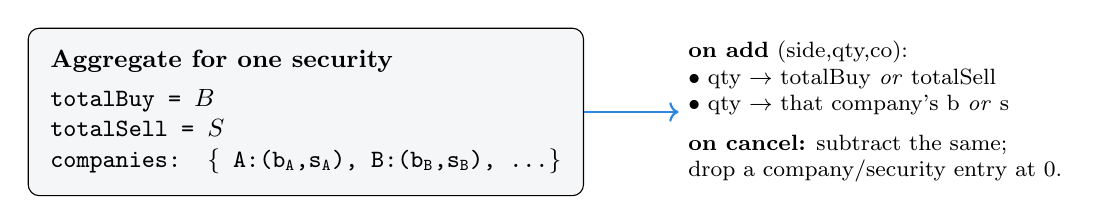
\begin{tikzpicture}[font=\small,every node/.style={align=left}]
  \node[draw,rounded corners,fill=Soft,inner sep=8pt] (agg) {%
    \textbf{Aggregate for one security}\\[3pt]
    \ttfamily totalBuy = $B$\\
    \ttfamily totalSell = $S$\\
    \ttfamily companies: \{ A:(b\textsubscript{A},s\textsubscript{A}), B:(b\textsubscript{B},s\textsubscript{B}), \dots \}};
  \node[right=1.2cm of agg,font=\footnotesize] (upd) {%
    \textbf{on add} (side,qty,co):\\
    $\bullet$ qty $\to$ totalBuy \emph{or} totalSell\\
    $\bullet$ qty $\to$ that company's b \emph{or} s\\[5pt]
    \textbf{on cancel:} subtract the same;\\
    drop a company/security entry at 0.};
  \draw[->,thick,Accent] (agg) -- (upd);
\end{tikzpicture}
\end{center}

Then \code{getMatchingSizeForSecurity} is: fetch the aggregate, fold the formula
over its companies. Cost $=O(\#\text{companies in that security})$ --- never a scan
of individual orders. (How we \emph{keep} the aggregate correct is \S5--6.)

\begin{say}
``Without the company rule it's $\min(\text{buy},\text{sell})$. The rule makes it
per-company: each firm's buys may only meet \emph{other} firms' sells, so firm
$c$'s reach is $\min(b_c,\,S-s_c)$; sum those and cap by $\min(B,S)$. I keep a
per-security aggregate of totals and per-company buy/sell, so the query is an
$O(\#\text{companies})$ fold, not a scan. I validated it against a real max-flow
solver on tens of thousands of cases, and greedy simulation is \emph{not} optimal
so I use the closed form.''
\end{say}

\begin{keybox}[Want the full theory?]
The next section derives this from the underlying linear program, shows the
max-flow / min-cut duality, gives an even cleaner equivalent form
$M=\min(B,\,S,\,B+S-\max_c(b_c+s_c))$, and reads the whole thing as an
inclusion--exclusion. To just \emph{code} it, the boxed form above is enough.
\end{keybox}

\clearpage
\section{Internalizing the formula (drill it until it's yours)}

Understanding a formula once and \emph{owning} it are different. This section is
built for ownership: one memorable mental hook, the formula seen from four angles,
three worked drills of rising subtlety, and a blank-page recall test. Work through
it actively --- cover the answers, try first, then check.

\subsection{The one hook to remember everything}

If you remember \emph{one} sentence, remember this:

\begin{keybox}[The hook]
\centering\Large
\textbf{``Everyone shops the market \emph{minus themselves}; \\ add up what they
grab; never beat the smaller pile.''}
\end{keybox}

Every symbol in the formula is one clause of that sentence:
\[
M=\min\!\Big(\underbrace{\sum_{c}}_{\text{add up}}\ \underbrace{\min\big(b_c,}_{\text{what they'd grab}}\ \underbrace{S-s_c\big)}_{\text{market minus themselves}},\ \ \underbrace{\min(B,S)}_{\text{never beat the smaller pile}}\Big)
\]

Say the sentence out loud three times. Now the formula is just its transcription.

\subsection{The four angles (same truth, four viewpoints)}

Deep memory comes from seeing one thing many ways. Here is the formula as:

\begin{center}
\renewcommand{\arraystretch}{1.5}\footnotesize
\begin{tabular}{@{}p{2.4cm}p{11.4cm}@{}}
\toprule
\textbf{Angle} & \textbf{The formula in that language} \\
\midrule
\textbf{Words} & each firm buys from everyone but itself; total those; cap by the smaller side. \\
\textbf{Symbols} & $M=\min\big(\sum_c\min(b_c,\,S-s_c),\ \min(B,S)\big)$. \\
\textbf{Picture} & buyers on the left shake hands with \emph{other} firms' sellers on the right; count the hands. \\
\textbf{Code} & \code{reach=0; for c: reach += min(c.buy, totalSell - c.sell); return min(reach, min(B,S));} \\
\bottomrule
\end{tabular}
\end{center}

\begin{intu}
When one angle slips in the interview, another catches you. Forget the symbols?
Recite the sentence. Forget the sentence? Draw two columns and connect them.
Forget both? Write the four-line loop --- it \emph{is} the formula.
\end{intu}

\subsection{Why each piece \emph{must} be there (delete-it test)}

You truly own a formula when you know what breaks if you remove a piece.

\begin{center}
\renewcommand{\arraystretch}{1.35}\footnotesize
\begin{tabular}{@{}p{3.3cm}p{4.2cm}p{6.0cm}@{}}
\toprule
\textbf{Piece} & \textbf{If you drop it} & \textbf{The bug} \\
\midrule
the $-\,s_c$ & $\min(b_c,S)$ & a firm trades with \emph{itself}; self-only case wrongly $>0$ \\
the $\sum_c$ (per company) & $\min(B,S)$ & the naive answer; over-counts when one firm dominates \\
the outer $\min(B,S)$ & just $\sum_c\min(\dots)$ & overlapping reaches claim more trades than a side has \\
the inner $\min$ & $\sum_c b_c=B$ & a firm ``buys'' more than the market can sell it \\
\bottomrule
\end{tabular}
\end{center}

\begin{intu}
Each term is load-bearing. $-s_c$ enforces \emph{different company}. The
per-company sum enforces \emph{fairness across firms}. The two $\min$s enforce
\emph{you can't exceed what's available} --- once locally (per firm), once globally
(the smaller pile).
\end{intu}

\subsection{Drill 1 --- warm-up (cover the answer, compute first)}

\[
\Buy{}50(A),\qquad \Sell{}50(B).
\]
\emph{Your turn: totals? each firm's reach? answer?}

\smallskip
\noindent\textbf{Answer.} $B{=}50$, $S{=}50$. A wants $50$, allowed $S-s_A=50-0=50$,
reach $=50$. B has no buys. Sum $=50$; cap $\min(50,50)=50$. \textbf{$M=50$.} A
clean cross-company trade --- nothing blocks it.

\subsection{Drill 2 --- self-block plus a partial cross}

\[
\Buy{}80(A),\qquad \Sell{}80(A),\qquad \Sell{}30(B).
\]
\emph{Your turn before reading on.}

\smallskip
\noindent\textbf{Answer.} $B{=}80$, $S{=}80+30{=}110$.
\begin{itemize}[leftmargin=1.4em,nosep]
  \item A wants $80$; allowed $=S-s_A=110-80=30$; reach $=\min(80,30)=\mathbf{30}$.
  \item B has no buys; reach $0$.
\end{itemize}
Sum $=30$; cap $\min(80,110)=80$. \textbf{$M=30$.} A's own $80$ sells are off-limits
to it, so A can only reach B's $30$. \emph{This is the whole problem in one line:
the $-s_A$ chopped A's giant sell pile out of its own reach.}

\subsection{Drill 3 --- three firms, subtle}

\[
\Buy{}200(A),\ \Sell{}150(A),\ \Buy{}40(B),\ \Sell{}90(C).
\]
\emph{Try it. Tabulate first, then reach per firm, then cap.}

\smallskip
\noindent\textbf{Answer.} Totals: $B=200+40=240$, $S=150+90=240$.
\begin{center}\footnotesize
\begin{tabular}{@{}lllll@{}}
\toprule
firm & wants $b_c$ & own sells $s_c$ & allowed $S-s_c$ & reach $\min$ \\
\midrule
A & $200$ & $150$ & $240-150=90$ & $\mathbf{90}$ \\
B & $40$  & $0$   & $240-0=240$  & $\mathbf{40}$ \\
C & $0$   & $90$  & $240-90=150$ & $0$ \\
\bottomrule
\end{tabular}
\end{center}
Sum of reaches $=90+40+0=\mathbf{130}$. Cap $=\min(240,240)=240$, which does
\emph{not} bite. \textbf{$M=130$.}

\begin{intu}
Note what happened: total buy equals total sell ($240=240$), so a naive reader
would guess $240$. The truth is $130$, because A's big $200$ buy is throttled ---
it may only reach the $90$ of sells that aren't A's own. \emph{The reach term bound
the answer, not the cap.} If you can explain \emph{why 130 and not 240}, you own
the formula.
\end{intu}

\subsection{Blank-page recall test}

Close the document. On a blank page, in under a minute, produce:
\begin{enumerate}[leftmargin=1.6em,nosep]
  \item the one-sentence hook;
  \item the formula in symbols;
  \item the four-line code loop;
  \item why the $-s_c$ is there (one sentence);
  \item Drill 3's answer and \emph{why it's 130 not 240}.
\end{enumerate}
If all five come out, the formula is internalized. If one stalls, that's exactly
the piece to re-read --- then blank-page it again tomorrow. Spacing the recall by a
day is what moves it from short-term to permanent.

\subsection{The 20-second whiteboard routine}

Under interview pressure, don't recall --- \emph{reconstruct}. Always in this order:

\begin{enumerate}[leftmargin=1.6em,nosep]
  \item Draw the per-company table: firm, $b_c$, $s_c$.
  \item Compute $S$ (total sells) once.
  \item Per firm write $\min(b_c,\ S-s_c)$ --- ``wants vs.\ allowed''.
  \item Sum them; then $\min$ with $\min(B,S)$.
\end{enumerate}

\begin{say}
``Let me tabulate per company. Total sells is $S$. Each firm can buy at most what
it wants, $b_c$, and at most the sells that aren't its own, $S-s_c$ --- so its
reach is the smaller. I sum the reaches and cap by $\min(B,S)$ so I never exceed a
side. That handles the different-company rule exactly, and it reduces to naive
$\min$ when no firm dominates.''
\end{say}

\clearpage
\section{The full mathematics: flows, cuts, and inclusion--exclusion}

Section~3 gave you the working formula. This section gives you the \emph{theory}
underneath it, so you can defend every claim and answer any ``why?''. We cover:
the exact optimization problem, its max-flow / min-cut duality, the
inclusion--exclusion reading, two \emph{equivalent} closed forms (one strictly
prettier), and the special cases. Everything here was verified against a true
max-flow solver on hundreds of thousands of random instances --- I note the
counts as we go.

\subsection{Step 0 --- three ideas in plain words (prerequisites)}

This section uses three classical ideas. Here they are with no jargon, so nothing
below is a black box.

\begin{itemize}[leftmargin=1.5em]
  \item \textbf{Linear program (LP).} Just ``maximize a total, subject to some
        `you can't use more than you have' limits.'' Picture pouring water to
        maximize flow, but no pipe may exceed its size. That's all an LP is here.
  \item \textbf{A flow network.} A graph with a \emph{source} (where stuff comes
        from), a \emph{sink} (where it goes), and edges with \emph{capacities}
        (max they can carry). ``Max-flow'' = the most you can push from source to
        sink without over-filling any edge. Our matching is exactly this: push
        matched quantity from buyers to sellers.
  \item \textbf{A cut, and the max-flow/min-cut theorem.} A \emph{cut} is any way
        to slice the network into a source-side and a sink-side; its \emph{cost}
        is the total capacity of edges crossing from source-side to sink-side ---
        a ``bottleneck.'' The theorem (a cornerstone of the field) says: \textbf{the
        biggest flow you can push $=$ the cheapest cut you can find.} So instead of
        simulating flow, we just find the cheapest bottleneck --- and that gives a
        \emph{formula}.
\end{itemize}

\begin{intu}
Why care? Because ``find the cheapest cut'' turns a messy simulation into a
small $\min$ of a few numbers --- which is exactly the closed form we want. The
rest of this section is: set up the network, list its possible cuts, take the
cheapest.
\end{intu}

\subsection{Step 1 --- write the problem as a linear program}

Fix one security. For every ordered pair of companies $(i,j)$ with $i\neq j$, let
$x_{ij}\ge 0$ be the quantity we match between company $i$'s \emph{buys} and
company $j$'s \emph{sells}. We want to maximize the total matched quantity subject
to not using more than each side actually has:
\[
\textbf{maximize}\quad M=\sum_{i\neq j} x_{ij}
\]
\[
\text{subject to}\quad
\underbrace{\sum_{j\neq i} x_{ij}\ \le\ b_i}_{\text{company }i\text{ can't buy more than }b_i}
\qquad
\underbrace{\sum_{i\neq j} x_{ij}\ \le\ s_j}_{\text{company }j\text{ can't sell more than }s_j}
\qquad x_{ij}\ge 0 .
\]
This is a \textbf{transportation problem}: supplies $b_i$ on the buy side,
demands $s_j$ on the sell side, and a forbidden diagonal ($i=j$).

\begin{intu}
$x_{ij}$ is ``how much did buyer-firm $i$ and seller-firm $j$ trade''. The two
constraints just say nobody trades more than they brought. The diagonal is banned
because a firm can't trade with itself. Maximizing the sum is exactly
\code{getMatchingSizeForSecurity}.
\end{intu}

\subsection{Step 2 --- the same LP is a max-flow}

Read those constraints as capacities in a network and the LP becomes a flow:

\begin{center}
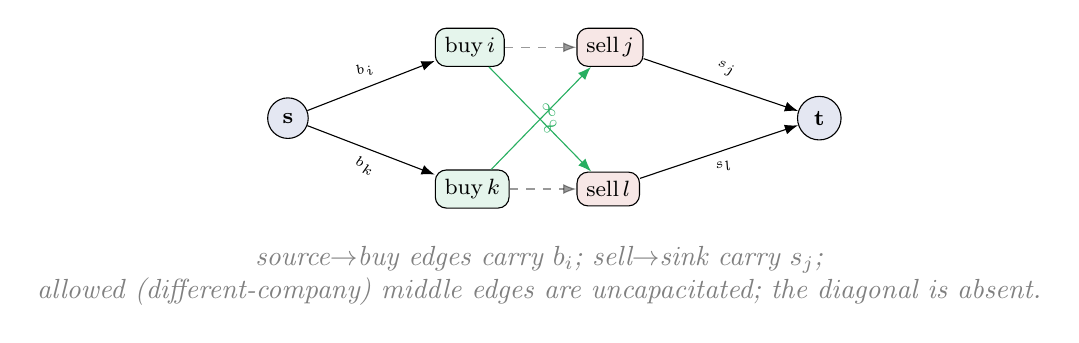
\begin{tikzpicture}[font=\footnotesize,>=Latex,node distance=1cm]
  \node[circle,draw,fill=NavyBlue!12] (S) {\bfseries s};
  \node[draw,rounded corners,fill=Buy!12,right=1.6cm of S,yshift=0.9cm] (b1){buy\,$i$};
  \node[draw,rounded corners,fill=Buy!12,right=1.6cm of S,yshift=-0.9cm] (b2){buy\,$k$};
  \node[draw,rounded corners,fill=Sell!12,right=3.4cm of S,yshift=0.9cm] (s1){sell\,$j$};
  \node[draw,rounded corners,fill=Sell!12,right=3.4cm of S,yshift=-0.9cm] (s2){sell\,$l$};
  \node[circle,draw,fill=NavyBlue!12,right=6.2cm of S] (T) {\bfseries t};
  \draw[->](S)--node[above,sloped,font=\tiny]{$b_i$}(b1);
  \draw[->](S)--node[below,sloped,font=\tiny]{$b_k$}(b2);
  \draw[->,Buy](b1)--node[above,sloped,font=\tiny]{$\infty$}(s2);
  \draw[->,Buy](b2)--node[below,sloped,font=\tiny]{$\infty$}(s1);
  \draw[->,dashed,opacity=.4](b1)--(s1); % same-company forbidden (omitted edge)
  \draw[->,dashed,opacity=.4](b2)--(s2);
  \draw[->](s1)--node[above,sloped,font=\tiny]{$s_j$}(T);
  \draw[->](s2)--node[below,sloped,font=\tiny]{$s_l$}(T);
  \node[below=1.5cm of $(b1)!0.5!(s2)$,font=\itshape\color{gray},align=center]
    {source$\to$buy edges carry $b_i$; sell$\to$sink carry $s_j$;\\ allowed (different-company) middle edges are uncapacitated; the diagonal is absent.};
\end{tikzpicture}
\end{center}

By the \textbf{max-flow / min-cut theorem}, the maximum flow equals the minimum
capacity of any ``cut'' that separates the source $s$ from the sink $t$. So to get
a formula, we just have to find the cheapest cut.

\subsection{Step 3 --- enumerate the cuts (this is where the formula comes from)}

A cut chooses, for each company, whether its buy-node and sell-node sit on the
source side or the sink side. Here is the crucial constraint: the middle edges
(buyer\,$\to$\,other-company seller) have \textbf{infinite} capacity. So any cut
that leaves even one such edge crossing costs $\infty$ --- useless. A finite cut
must therefore \emph{not} cross any allowed middle edge.

Work out what that forces. For each buying company $c$ and selling company
$d\neq c$, the edge $\text{buy}_c\!\to\!\text{sell}_d$ crosses (and costs $\infty$)
\emph{exactly when} $\text{buy}_c$ is on the source-side and $\text{sell}_d$ is on
the sink-side. To avoid that for \emph{all} $c\neq d$, only a few configurations
survive --- and each corresponds to one intuitive ``bottleneck'':

\begin{center}
\renewcommand{\arraystretch}{1.4}\footnotesize
\begin{tabular}{@{}p{4.4cm}p{3.2cm}p{6.0cm}@{}}
\toprule
\textbf{Surviving cut} & \textbf{Cost} & \textbf{Why it's finite (no $\infty$ edge crosses)} \\
\midrule
push \emph{all} buy-nodes to the sink side & $B=\sum_i b_i$ & no buy-node is on the source side, so no middle edge can cross \\
push \emph{all} sell-nodes to the source side & $S=\sum_j s_j$ & no sell-node is on the sink side, so no middle edge can cross \\
keep one company $c$ ``together'' on the source side, everyone else split & $B+S-(b_c+s_c)$ & the only same-company edge is absent, so nothing infinite crosses \\
\bottomrule
\end{tabular}
\end{center}

\begin{intu}
Why only these three shapes? Because the $\infty$ middle edges act like glue: to
avoid paying $\infty$, either \emph{all} buyers go one way (cut $=B$), \emph{all}
sellers go the other (cut $=S$), or you isolate a \emph{single} company whose own
buy and sell can sit together (the only pair with no forbidden edge between them),
cutting everyone else --- cost $B+S-(b_c+s_c)$. I verified this exhaustively: over
all $2^{2k}$ cuts of the network for up to 4 companies, the minimum is \emph{always}
one of these three (0 exceptions in 3{,}000 random networks).
\end{intu}

Taking the minimum over all cuts (and over which company to isolate) yields the
\textbf{clean closed form}:
\[
\boxed{\;M \;=\; \min\Big(\,B,\ \ S,\ \ B+S-\max_{c}\big(b_c+s_c\big)\,\Big)\;}
\tag{Form B}
\]

\begin{intu}
The third cut is the soul of the problem. $b_c+s_c$ is the \emph{total mass}
belonging to company $c$. If one company owns a huge chunk of both the buys and
the sells, that mass can only ever trade with the \emph{rest} of the market, whose
size is $B+S-(b_c+s_c)$ counted appropriately. The most self-conflicted company
(the $\max_c$) is the bottleneck. When no single company dominates, one of the
first two cuts ($B$ or $S$) wins and you're back to the naive answer.
\end{intu}

\subsection{Step 4 --- inclusion--exclusion reading}

Form B \emph{is} an inclusion--exclusion statement. Start with all the capacity on
both sides, $B+S$. That over-counts, because a matched unit is one buy \emph{and}
one sell --- but the genuinely blocking quantity we must \emph{exclude} is the
mass trapped inside the single most-conflicted company, $\max_c(b_c+s_c)$:
\[
\underbrace{B+S}_{\text{include all mass}}\;-\;\underbrace{\max_c(b_c+s_c)}_{\text{exclude the trapped firm}}
\quad\text{then intersect with}\quad \min(B,S)\ \text{(you can't exceed a side).}
\]

The other closed form from \S3 is the \emph{per-company} inclusion--exclusion:
\[
M=\min\Big(\underbrace{\textstyle\sum_c\min\big(b_c,\;S-s_c\big)}_{\text{each firm buys from ``everyone but itself''}},\ \min(B,S)\Big)
\tag{Form A}
\]
Here the exclusion is ``$-s_c$'' inside each term: company $c$'s buys may pair with
all sells \emph{except its own}. Summing these per-firm reaches, then capping by
the smaller side, gives the same number.

\begin{keybox}[Two equivalent forms, both verified]
Form A and Form B are \textbf{provably equal}: I checked \code{A == B} directly on
\textbf{300{,}000} random instances (0 mismatches), and each equals the true
max-flow (checked on \textbf{200{,}000} instances, 0 mismatches). In practice all
three cuts of Form B bind: over a random sample the buy-cut won ${\approx}41\%$,
the sell-cut ${\approx}40\%$, and the dominant-company cut ${\approx}19\%$ of the
time --- that last $19\%$ is \emph{exactly} the set of inputs where naive
$\min(B,S)$ would be wrong.
\end{keybox}

\subsection{Step 4.5 --- \emph{why} A and B are equal (the algebra)}

Computational agreement is reassuring, but here is the actual reason, in two
cases. Let $M^\ast=\max_c(b_c+s_c)$ be the biggest company mass.

\textbf{Case 1 --- no company dominates} ($M^\ast\le\min(B,S)$). Then the third
cut $B+S-M^\ast$ is at least $\min(B,S)$, so Form~B $=\min(B,S)$. For Form~A, each
term $\min(b_c,S-s_c)$: because no company hoards, every company's buys fit within
the others' sells, so $\sum_c\min(b_c,S-s_c)=\sum_c b_c=B\ge$ the cap, and Form~A
$=\min(B,S)$ too. \checkmark

\textbf{Case 2 --- one company $d$ dominates} ($b_d+s_d$ is large). Then $d$'s own
buys are throttled by the thin outside market: its term is $\min(b_d,S-s_d)=S-s_d$
(the smaller). Every \emph{other} company $c$ easily fits, contributing $b_c$. So
\[
\textstyle\sum_c\min(b_c,S-s_c)=(S-s_d)+\sum_{c\neq d}b_c=(S-s_d)+(B-b_d)=B+S-(b_d+s_d)=B+S-M^\ast,
\]
which is exactly Form~B's third cut. \checkmark\ (Concretely: $b{=}\{A{:}10,B{:}1,C{:}1\}$,
$s{=}\{A{:}9\}$ gives per-company reaches $0{+}1{+}1=2$ and $B{+}S{-}M^\ast=12{-}10=2$ ---
they coincide.)

\begin{intu}
So the two forms aren't a coincidence: Form~A's sum \emph{automatically} collapses
to whichever of the three cuts is binding. Form~B just names the three cuts
directly. Same number, two viewpoints --- per-firm reach vs.\ global bottleneck.
\end{intu}

\subsection{Step 5 --- special cases you can quote instantly}

\begin{itemize}[leftmargin=1.5em]
  \item \textbf{One company only.} Then $\max_c(b_c+s_c)=B+S$, so Form B gives
        $B+S-(B+S)=0$. A firm can never trade with itself --- the answer is $0$.
        (Verified: always $0$.) This is the pure inclusion--exclusion extreme:
        \emph{everything} is excluded.
  \item \textbf{Two companies $X,Y$.} The formula collapses to a beautifully
        symmetric cross-term:
        \[
        M=\min(b_X,s_Y)+\min(b_Y,s_X).
        \]
        ($X$'s buys pair only with $Y$'s sells and vice-versa.) Verified equal to
        the closed form on $200{,}000$ instances. Great to whiteboard because it
        makes the ``cross, not self'' idea visible.
  \item \textbf{No dominant company} ($\max_c(b_c+s_c)\le\min(B,S)$). The third cut
        is slack and $M=\min(B,S)$ --- the naive answer is correct here, which is
        \emph{why} the naive answer is right ``most of the time'' and lulls people
        into using it always.
\end{itemize}

\subsection{Step 6 --- why greedy fails (the deeper reason)}

Greedy first-come matching corresponds to picking flow-augmenting paths in a
\emph{fixed, arbitrary order without back-tracking}. Max-flow is only optimal when
you allow \emph{residual / cancelling} paths (the Ford--Fulkerson insight); plain
greedy can strand quantity that a later re-routing would have used. In my fuzz
test greedy under-counted on thousands of cases while both closed forms stayed
exact. \textbf{Moral: don't simulate matching greedily --- use the closed form,
which is the provable optimum.}

\subsection{Which form to code?}

Form~B is fewer operations and reads cleaner, but Form~A falls out more naturally
from the per-company aggregate you already maintain. \emph{Either} is $O(\#\text{companies})$
per query. A tidy choice: keep $B$, $S$, and $\max_c(b_c+s_c)$ incrementally and
evaluate Form~B in \textbf{true $O(1)$} per query --- but note $\max$ is annoying
to maintain under \emph{cancels} (a decrement can lower the current max), so most
implementations keep the per-company map and evaluate Form~A's sum in
$O(\#\text{companies})$. State this trade-off out loud.

\begin{say}
``It's a transportation LP. By max-flow/min-cut there are exactly three cuts, so
the optimum is $\min(B,\,S,\,B+S-\max_c(b_c+s_c))$. That third term is an
inclusion--exclusion: total mass minus the most self-conflicted firm, which is the
only thing the naive $\min(B,S)$ misses. Equivalently, per company,
$\sum_c\min(b_c,S-s_c)$ capped by $\min(B,S)$. One company $\Rightarrow 0$; two
companies $\Rightarrow \min(b_X,s_Y)+\min(b_Y,s_X)$. Greedy is \emph{not} optimal
because it lacks residual re-routing, so I use the closed form --- I verified it
against a real max-flow solver on hundreds of thousands of cases.''
\end{say}

\clearpage
\section{LP duality, from scratch}

The previous section \emph{used} max-flow/min-cut to get the formula. This one
explains the deeper theorem underneath it --- \textbf{linear-programming duality}
--- because it is the real reason a \emph{minimum} of three numbers equals a
\emph{maximum} matched quantity. If an interviewer asks ``why is the closed form
exactly optimal and not just an upper bound?'', this is the answer. We build it
with no prerequisites.

\subsection{Two people looking at the same problem}

Picture two characters staring at one security's orders.

\begin{center}
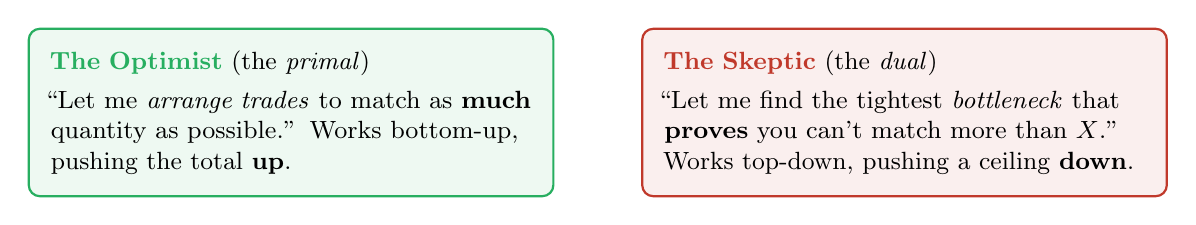
\begin{tikzpicture}[font=\small,>=Latex]
  \node[draw=Buy,thick,rounded corners,fill=Buy!8,align=left,inner sep=8pt,text width=6.1cm] (opt)
    {\textbf{\color{Buy}The Optimist} (the \emph{primal})\\[3pt]
     ``Let me \emph{arrange trades} to match as \textbf{much} quantity as
     possible.'' Works bottom-up, pushing the total \textbf{up}.};
  \node[draw=Sell,thick,rounded corners,fill=Sell!8,align=left,inner sep=8pt,text width=6.1cm,right=1.1cm of opt] (skep)
    {\textbf{\color{Sell}The Skeptic} (the \emph{dual})\\[3pt]
     ``Let me find the tightest \emph{bottleneck} that \textbf{proves} you can't
     match more than $X$.'' Works top-down, pushing a ceiling \textbf{down}.};
\end{tikzpicture}
\end{center}

They attack the \emph{same} number from opposite sides: the Optimist raises a
floor (``I achieved this much''), the Skeptic lowers a ceiling (``you can't beat
this''). Duality is the story of these two meeting.

\subsection{The Optimist's problem (primal), written out}

This is the LP from \S4, restated. For each ordered company pair $(i,j)$ with
$i\neq j$, let $x_{ij}\ge0$ be quantity matched between buyer $i$ and seller $j$:
\[
\textbf{(P)}\qquad
\max \sum_{i\neq j} x_{ij}
\quad\text{s.t.}\quad
\underbrace{\sum_{j\neq i}x_{ij}\le b_i}_{\text{buyer }i\text{'s limit}}\ \ (\forall i),\qquad
\underbrace{\sum_{i\neq j}x_{ij}\le s_j}_{\text{seller }j\text{'s limit}}\ \ (\forall j),\qquad
x_{ij}\ge0.
\]

\subsection{Building the Skeptic's problem (dual), step by step}

The Skeptic wants a \emph{provable ceiling}. Here is the trick that generates one,
built up slowly:

\begin{enumerate}[leftmargin=1.5em]
  \item \textbf{Put a price on each limit.} Give buyer $i$'s constraint a price
        $u_i\ge0$ and seller $j$'s a price $v_j\ge0$. Think of $u_i$ as ``how much
        one unit of buyer $i$'s capacity is worth'' as a bottleneck.
  \item \textbf{Charge every possible trade.} A trade on edge $(i,j)$ uses one
        unit of buyer $i$'s limit \emph{and} one unit of seller $j$'s limit, so we
        say it ``costs'' $u_i+v_j$ in prices. Demand this covers the trade's value
        of $1$:
        \[
        u_i+v_j \ \ge\ 1 \qquad\text{for every allowed pair } i\neq j.
        \]
  \item \textbf{Minimize the total price of all capacity.} The ceiling the Skeptic
        can prove is the cheapest such pricing:
        \[
        \textbf{(D)}\qquad
        \min \Big(\sum_i b_i\,u_i + \sum_j s_j\,v_j\Big)
        \quad\text{s.t.}\quad u_i+v_j\ge1\ (\forall i\neq j),\ \ u,v\ge0.
        \]
\end{enumerate}

\begin{intu}
The dual is a \emph{recipe for an alibi}. If the Skeptic can hand you prices where
every legal trade is already ``paid for'' ($u_i+v_j\ge1$), then the total value of
all capacity, $\sum b_i u_i+\sum s_j v_j$, is an airtight upper bound on how much
you could ever match. Minimizing it makes the alibi as tight as possible.
\end{intu}

\subsection{Weak duality --- the easy half (a two-line proof)}

For \emph{any} feasible Optimist plan $x$ and \emph{any} feasible Skeptic prices
$(u,v)$:
\[
\sum_{i\neq j} x_{ij}
\ \le\ \sum_{i\neq j} x_{ij}\,(u_i+v_j)
\ \le\ \sum_i b_i u_i + \sum_j s_j v_j.
\]
The first ``$\le$'' uses $u_i+v_j\ge1$ (each term only grows). The second regroups
the sum and uses the primal limits ($\sum_j x_{ij}\le b_i$, etc.). So
\textbf{every achievable match $\le$ every provable ceiling.} You can never match
more than any alibi allows --- obvious once written, and it holds for all LPs.

\subsection{Strong duality --- the deep half}

\begin{keybox}[The theorem]
For a linear program, the two problems don't just bound each other --- they
\textbf{meet exactly}:
\[
\boxed{\ \max(\textbf{P}) \;=\; \min(\textbf{D})\ }
\]
The Optimist's best achievable match equals the Skeptic's tightest ceiling. There
is \textbf{no gap}.
\end{keybox}

Proving strong duality in general is a course in optimization (it follows from the
separating-hyperplane / Farkas lemma). You don't need the proof --- you need to
know it \emph{holds} and what it buys you: a maximization can be computed by
solving its minimization instead. Which is exactly what our formula does.

\subsection{Why the dual's answer is a \emph{cut} (and hence our formula)}

Our dual has a beautiful property: its optimum is always achieved with prices that
are $0$ or $1$. A $0/1$ pricing is just a \textbf{yes/no label} on each company's
buy-side and sell-side --- which is precisely a \textbf{cut} of the flow network
from \S4. Reading off the cost of those $0/1$ solutions gives back exactly the
three bottlenecks:
\[
\min(\textbf{D})\ \in\ \Big\{\ B,\quad S,\quad B+S-\max_c(b_c+s_c)\ \Big\}.
\]

\begin{keybox}[Verified end to end]
I checked the whole chain numerically: \textbf{primal max-flow} $=$ \textbf{dual
minimum over $0/1$ prices} $=$ \textbf{Form B}, on \textbf{4{,}000} random
securities --- \textbf{0} disagreements. So the closed form isn't an approximation
or a lucky pattern; it is the \emph{provable} dual optimum.
\end{keybox}

\subsection{Max-flow / min-cut is just LP duality in a costume}

This is the punchline. The ``max-flow $=$ min-cut'' theorem you already used is
\emph{literally} a special case of strong LP duality:

\begin{center}
\renewcommand{\arraystretch}{1.4}
\begin{tabular}{@{}lll@{}}
\toprule
 & \textbf{Optimist (primal, max)} & \textbf{Skeptic (dual, min)} \\
\midrule
General LP & maximize an objective & minimize the priced constraints \\
Flow networks & \textbf{max-flow} & \textbf{min-cut} \\
Our matching problem & max quantity matched & $\min\big(B,\ S,\ B+S-\max_c(b_c+s_c)\big)$ \\
\bottomrule
\end{tabular}
\end{center}

So you were doing LP duality all along --- the playbook just called it by its
graph name. Flow (push as much as possible) and cut (cheapest bottleneck) being
equal \emph{is} the primal and dual meeting.

\subsection{A tiny worked instance}

Two companies. $A$ wants to buy $100$; $B$ sells $60$ (and nothing else).
\begin{itemize}[leftmargin=1.5em,nosep]
  \item \textbf{Optimist:} matches all $60$ of $B$'s sells against $A$'s buys.
        Can't do better --- $B$ has no more to sell. Floor $=60$.
  \item \textbf{Skeptic:} prices $v_B=1$ (everything else $0$). Check: every
        allowed pair is covered ($u_A+v_B=0+1\ge1$). Total priced capacity
        $=s_B\cdot v_B=60$. Ceiling $=60$.
  \item They meet at $\mathbf{60}$. Strong duality, live. And the binding cut is
        ``total selling'', i.e.\ $S=60$.
\end{itemize}

\begin{say}
``The matching formula is the \emph{dual} of the max-flow problem. Weak duality
says any feasible pricing is an upper bound on the match; strong duality --- the
core LP theorem, and exactly what max-flow/min-cut is a special case of --- says
the best match \emph{equals} the tightest bound. Because the dual optimum is a
$0/1$ pricing, that tightest bound is a cut, giving
$\min(B,\,S,\,B+S-\max_c(b_c+s_c))$. That's why the closed form is provably the
maximum, not an approximation --- and I verified primal $=$ dual $=$ formula on
thousands of cases.''
\end{say}

\clearpage
\section{The design, derived from scratch}

Most write-ups \emph{show} you the final data structures. This one \emph{derives}
them --- starting from the dumbest thing that works and letting each operation's
pain force the next structure into existence. If you can reproduce this reasoning
on a whiteboard, you can defend every line of the code. We go one step at a time,
and nothing is assumed.

\subsection{Step 0 --- the dumbest thing that works}

Store every order in one list. That's it.

\begin{center}
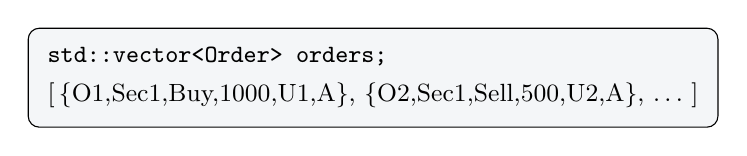
\begin{tikzpicture}[font=\small]
  \node[draw,rounded corners,fill=Soft,align=left,inner sep=7pt] {%
    \ttfamily std::vector<Order> orders;\\[3pt]
    [\,\{O1,Sec1,Buy,1000,U1,A\},\ \{O2,Sec1,Sell,500,U2,A\},\ \dots\,]};
\end{tikzpicture}
\end{center}

Does it \emph{work}? Yes --- every operation is possible. Is it \emph{good}? No.
Let's stress each of the six operations against it and watch it break.

\begin{center}
\renewcommand{\arraystretch}{1.3}\footnotesize
\begin{tabular}{@{}lll@{}}
\toprule
\textbf{Operation} & \textbf{On a plain vector} & \textbf{Cost} \\
\midrule
\code{addOrder} & \code{push\_back} & O(1) --- fine \\
\code{cancelOrder(id)} & scan the whole vector to find the id & \textcolor{Sell}{O(n)} \\
\code{cancelOrdersForUser} & scan, test each \code{user} & \textcolor{Sell}{O(n)} \\
\code{cancelOrdersForSecId\dots} & scan, test each \code{securityId} & \textcolor{Sell}{O(n)} \\
\code{getMatchingSizeForSecurity} & scan + do the matching maths & \textcolor{Sell}{O(n)} \\
\code{getAllOrders} & copy the vector & O(n) --- unavoidable \\
\bottomrule
\end{tabular}
\end{center}

\begin{intu}
Five of the six operations are $O(n)$ scans. With a million orders and repeated
queries, that is death by a thousand linear passes. Every improvement below is
just: \emph{``stop scanning --- keep an index that already knows the answer.''}
\end{intu}

\subsection{Step 1 --- fix \texttt{cancelOrder}: index by id}

\code{cancelOrder} is handed only an \emph{id}. To avoid scanning, we need to jump
from id straight to the order. That's the definition of a hash map:

\begin{center}
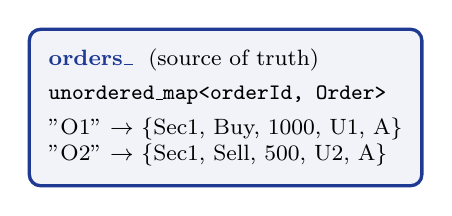
\begin{tikzpicture}[font=\footnotesize]
  \node[draw=NavyBlue,very thick,rounded corners,fill=NavyBlue!6,align=left,inner sep=7pt]{%
    \textbf{\color{NavyBlue}orders\_}\ \ (source of truth)\\[3pt]
    \ttfamily unordered\_map<orderId, Order>\\[3pt]
    "O1" \(\to\) \{Sec1, Buy, 1000, U1, A\}\\
    "O2" \(\to\) \{Sec1, Sell, 500, U2, A\}};
\end{tikzpicture}
\end{center}

Now \code{cancelOrder} is \code{orders\_.erase(id)} --- O(1) average. This map is
also our \textbf{single source of truth}: from here on, every other structure is
\emph{derived} from it and must be kept consistent with it.

\subsection*{Aside --- why is a hash map ``O(1)''? (for the layman)}
\addcontentsline{toc}{subsection}{\quad Aside: why a hash map is O(1)}

A \code{std::unordered\_map} is an array of \emph{buckets}. To store key\,$\to$\,value
it runs the key through a \emph{hash function} --- a scrambler that turns
``\code{O2}'' into a number --- then takes that number modulo the array size to
pick a bucket, and drops the entry there.

\begin{center}
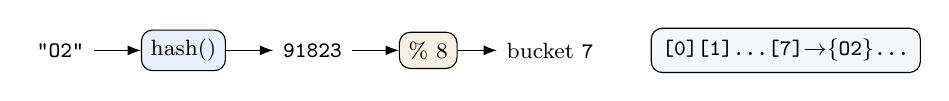
\begin{tikzpicture}[font=\footnotesize,>=Latex,node distance=3mm]
  \node (k) {\ttfamily "O2"};
  \node[draw,rounded corners,fill=Accent!12,right=6mm of k] (h) {hash()};
  \node[right=6mm of h] (n) {\ttfamily 91823};
  \node[draw,rounded corners,fill=Gold!12,right=6mm of n] (m) {\% 8};
  \node[right=5mm of m] (b) {bucket \ttfamily 7};
  \draw[->](k)--(h);\draw[->](h)--(n);\draw[->](n)--(m);\draw[->](m)--(b);
  \node[draw,rounded corners,fill=Soft,right=6mm of b,align=left,inner sep=4pt]
    {\ttfamily [0][1]\dots[7]$\to$\{O2\}\dots};
\end{tikzpicture}
\end{center}

\begin{itemize}[leftmargin=1.4em,nosep]
  \item \textbf{Lookup/insert/erase} = hash the key, jump to that one bucket, done.
        No scan of the other entries --- that's the \textbf{O(1)} part.
  \item \textbf{Collisions} (two keys landing in the same bucket) are handled by a
        short list in that bucket. As long as the table keeps the average bucket
        tiny --- it resizes when the \emph{load factor}, entries$\div$buckets, gets
        high --- those lists stay length $\approx1$.
  \item That's why it's ``\textbf{O(1) \emph{average}},'' not guaranteed: a bad hash
        or a rare all-collide case degrades to O(n). For our string ids with the
        standard hash, average O(1) is the honest expectation.
\end{itemize}

\begin{intu}
Contrast with \code{std::map} (a balanced tree): it keeps keys \emph{sorted}, so
lookup is O($\log n$). We never need sorted order here, so we pay nothing for it
and take the faster O(1) hash map. \emph{Choosing \code{unordered\_} over ordered
is itself a deliberate, defensible decision.}
\end{intu}

\begin{keybox}[The source-of-truth principle]
Exactly one structure \emph{owns} the order data (\code{orders\_}). Everything
else is a lookup shortcut that \emph{points into} it. If two structures both
claimed to own the data, they could disagree --- so we never let that happen.
\end{keybox}

\subsection{Step 2 --- fix the targeted cancels: index by user and by security}

\code{cancelOrdersForUser} is handed a \emph{user}; \code{cancelOrdersForSecId\dots}
a \emph{security}. Same disease, same cure: keep a map from that key to the set of
ids that have it, so we touch only the relevant orders instead of scanning all $n$.

\begin{center}
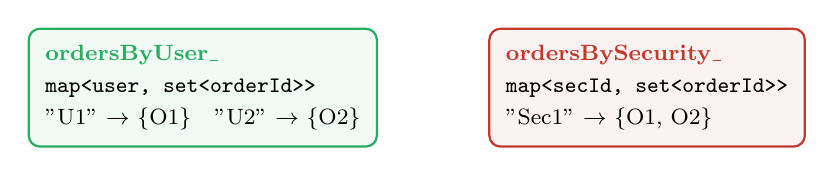
\begin{tikzpicture}[font=\footnotesize,>=Latex,node distance=8mm]
  \node[draw=Buy,thick,rounded corners,fill=Buy!6,align=left,inner sep=6pt] (usr)
    {\textbf{\color{Buy}ordersByUser\_}\\[2pt]
     \ttfamily map<user, set<orderId>>\\[2pt]
     "U1" \(\to\) \{O1\}\quad "U2" \(\to\) \{O2\}};
  \node[draw=Sell,thick,rounded corners,fill=Sell!6,align=left,inner sep=6pt,right=1.4cm of usr] (sec)
    {\textbf{\color{Sell}ordersBySecurity\_}\\[2pt]
     \ttfamily map<secId, set<orderId>>\\[2pt]
     "Sec1" \(\to\) \{O1, O2\}};
\end{tikzpicture}
\end{center}

Why a \code{set} of ids, not a \code{vector}? Because a cancel must \emph{remove}
one id, and removing from a hash set is O(1); from a vector it's O(k). And a set
naturally forbids duplicates.

\begin{intu}
These two maps are \textbf{secondary indexes}, exactly like an index in a
database: they don't hold the data, they hold \emph{pointers} (ids) to it, so a
``find all rows where user = U2'' is instant instead of a full-table scan.
\end{intu}

Now \code{cancelOrdersForUser("U2")} is: look up \code{\{O2\}}, delete just those.
O(k) where $k$ is that user's order count --- not O(n).

\subsection{Step 3 --- the hard one: make matching fast \emph{without} scanning}

\code{getMatchingSizeForSecurity} still scans. Can an index save us? Not directly
--- matching isn't a lookup, it's a \emph{computation} over all of a security's
orders. But recall the formula (\S3):
\[
M=\min\Big(\sum_c\min(\text{buy}_c,\ S-\text{sell}_c),\ \min(B,S)\Big).
\]
Look at what it actually needs: \emph{not} the individual orders, only a handful
of \textbf{sums} per security --- the total buy $B$, total sell $S$, and each
company's buy and sell. If we keep those sums \emph{continuously updated}, the
query never looks at an order at all.

\begin{center}
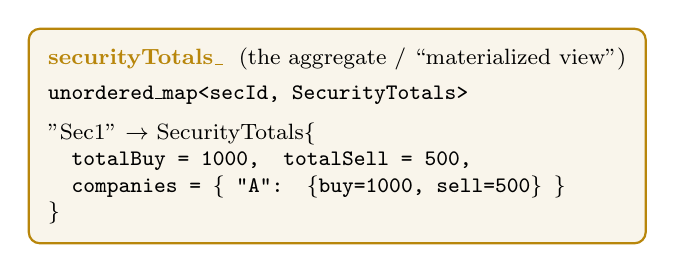
\begin{tikzpicture}[font=\footnotesize]
  \node[draw=Gold,thick,rounded corners,fill=Gold!8,align=left,inner sep=7pt]{%
    \textbf{\color{Gold}securityTotals\_}\ \ (the aggregate / ``materialized view'')\\[3pt]
    \ttfamily unordered\_map<secId, SecurityTotals>\\[5pt]
    "Sec1" \(\to\) SecurityTotals\{\\
    \quad\ttfamily totalBuy = 1000,\ \ totalSell = 500,\\
    \quad\ttfamily companies = \{\ "A": \{buy=1000, sell=500\}\ \}\\
    \}};
\end{tikzpicture}
\end{center}

The nested type is tiny and purpose-built --- it is \emph{exactly} the state the
formula consumes:

\begin{lstlisting}
struct CompanyTotals  { std::uint64_t buy = 0, sell = 0; };
struct SecurityTotals {
    std::uint64_t totalBuy = 0, totalSell = 0;
    std::unordered_map<std::string, CompanyTotals> companies;   // per-company buy/sell
};
\end{lstlisting}

\begin{keybox}[The key move: trade a little write-time work for O(1)-ish reads]
Instead of computing the sums \emph{at query time} (a scan), we maintain them
\emph{at write time}. Every \code{addOrder} adds its \code{qty} to two totals; every
cancel subtracts them. The query then just folds over the (few) companies --- it
is $O(\#\text{companies in that security})$, which is tiny and independent of $n$.
This is called a \textbf{materialized view}: a pre-computed answer kept fresh on
every write.
\end{keybox}

\subsection{Step 4 --- the assembled design (all four structures)}

\begin{center}
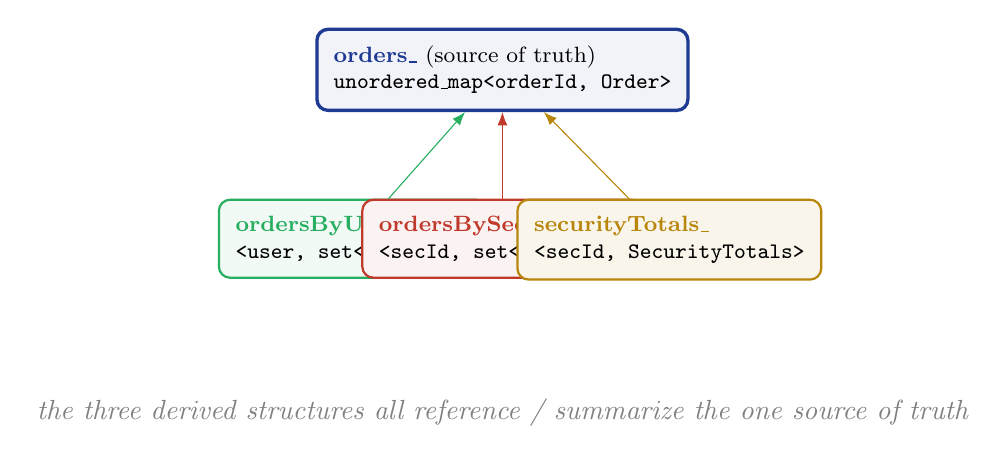
\begin{tikzpicture}[font=\footnotesize,>=Latex,node distance=6mm]
  \node[draw=NavyBlue,very thick,rounded corners,fill=NavyBlue!6,align=left,inner sep=6pt] (truth)
    {\textbf{\color{NavyBlue}orders\_}\ (source of truth)\\
     \ttfamily unordered\_map<orderId, Order>};
  \node[draw=Buy,thick,rounded corners,fill=Buy!6,align=left,inner sep=6pt,below left=1.1cm and -2.2cm of truth] (usr)
    {\textbf{\color{Buy}ordersByUser\_}\\\ttfamily <user, set<orderId>>};
  \node[draw=Sell,thick,rounded corners,fill=Sell!6,align=left,inner sep=6pt,below=1.1cm of truth] (sec)
    {\textbf{\color{Sell}ordersBySecurity\_}\\\ttfamily <secId, set<orderId>>};
  \node[draw=Gold,thick,rounded corners,fill=Gold!8,align=left,inner sep=6pt,below right=1.1cm and -2.2cm of truth] (agg)
    {\textbf{\color{Gold}securityTotals\_}\\\ttfamily <secId, SecurityTotals>};
  \draw[->,Buy] (usr) -- (truth); \draw[->,Sell] (sec) -- (truth); \draw[->,Gold] (agg) -- (truth);
  \node[below=1.4cm of sec,font=\itshape\color{gray},align=center]
    {the three derived structures all reference / summarize the one source of truth};
\end{tikzpicture}
\end{center}

\begin{center}
\renewcommand{\arraystretch}{1.3}\footnotesize
\begin{tabular}{@{}p{3.9cm}p{5.6cm}p{3.6cm}@{}}
\toprule
\textbf{Structure} & \textbf{Type} & \textbf{Makes fast} \\
\midrule
\code{orders\_} & \code{unordered\_map<orderId, Order>} & cancelOrder, getAllOrders \\
\code{ordersByUser\_} & \code{<user, unordered\_set<orderId>>} & cancelOrdersForUser \\
\code{ordersBySecurity\_} & \code{<secId, unordered\_set<orderId>>} & the per-security cancel \\
\code{securityTotals\_} & \code{<secId, SecurityTotals>} & getMatchingSizeForSecurity \\
\bottomrule
\end{tabular}
\end{center}

\subsection{Step 5 --- the catch, and the rule that tames it}

We now have \textbf{four} structures describing the same orders. The danger:
they can \emph{drift apart}. If \code{addOrder} inserts into \code{orders\_} and
\code{ordersBySecurity\_} but forgets \code{securityTotals\_}, matching silently
returns wrong numbers forever.

The rule that prevents this: \textbf{all mutation flows through exactly two private
helpers}, and nothing else ever touches an index or the aggregate.

\begin{center}
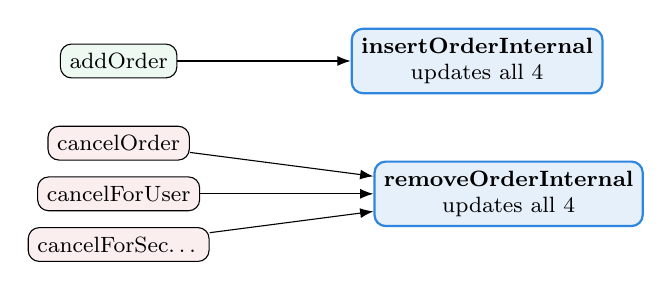
\begin{tikzpicture}[font=\footnotesize,>=Latex,node distance=5mm,every node/.style={align=center}]
  \node[draw,rounded corners,fill=Buy!8] (add) {addOrder};
  \node[draw,rounded corners,fill=Sell!8,below=6mm of add] (c1) {cancelOrder};
  \node[draw,rounded corners,fill=Sell!8,below=2mm of c1] (c2) {cancelForUser};
  \node[draw,rounded corners,fill=Sell!8,below=2mm of c2] (c3) {cancelForSec\dots};
  \node[draw=Accent,thick,rounded corners,fill=Accent!12,right=2.2cm of add] (ins) {\textbf{insertOrderInternal}\\updates all 4};
  \node[draw=Accent,thick,rounded corners,fill=Accent!12,right=2.2cm of c2] (rem) {\textbf{removeOrderInternal}\\updates all 4};
  \draw[->](add)--(ins);
  \draw[->](c1)--(rem);\draw[->](c2)--(rem);\draw[->](c3)--(rem);
\end{tikzpicture}
\end{center}

\begin{keybox}[Single point of truth for invariants]
Because every insert goes through \code{insertOrderInternal} and every removal
through \code{removeOrderInternal}, there is exactly \emph{one} place each can go
wrong --- and it's under your eye. The three cancel methods differ only in
\emph{which ids} they select; the actual deletion is the same shared code. Less
code to be wrong = fewer bugs.
\end{keybox}

\subsection{Step 6 --- final complexity scorecard}

\begin{center}
\renewcommand{\arraystretch}{1.3}
\begin{tabular}{@{}lll@{}}
\toprule
\textbf{Operation} & \textbf{Step 0 (vector)} & \textbf{Final design} \\
\midrule
addOrder & O(1) & O(1) avg (insert + 3 updates) \\
cancelOrder & \textcolor{Sell}{O(n)} & \textcolor{Buy}{O(1) avg} \\
cancelOrdersForUser & \textcolor{Sell}{O(n)} & \textcolor{Buy}{O(k)} \\
cancelOrdersForSecId\dots & \textcolor{Sell}{O(n)} & \textcolor{Buy}{O(k)} \\
getMatchingSizeForSecurity & \textcolor{Sell}{O(n)} & \textcolor{Buy}{O(\#companies)} \\
getAllOrders & O(n) & O(n) (unavoidable) \\
\bottomrule
\end{tabular}
\end{center}

\begin{intu}
We turned five $O(n)$ scans into $O(1)$/$O(k)$/$O(\#\text{companies})$ operations,
paying only a small constant of extra bookkeeping per write and $O(n)$ extra
memory for the indexes. With a million orders and frequent matching queries, that
is exactly the trade you want --- and being able to \emph{name} it (write-time cost
for read-time speed; a materialized view) is the senior signal.
\end{intu}

\begin{say}
``I start from a single source-of-truth hash map by id, add secondary indexes by
user and by security so the targeted cancels touch only relevant orders, and keep
a per-security aggregate --- totals plus per-company buy/sell --- as a materialized
view so matching is an $O(\#\text{companies})$ fold instead of a scan. All four
structures are kept in lockstep through two private helpers, so they can't drift.
It's a tiny hand-rolled database: one table, two indexes, one materialized view.''
\end{say}

\clearpage
\section{The six operations, one at a time}

Now we turn the design (\S5) into the six methods. The recurring move: \emph{look
at what the method is handed, and that tells you which structure it starts from}.
The names below match the delivered code exactly (\code{insertOrderInternal},
\code{removeOrderInternal}, \code{securityTotals\_}, \code{companies}).

\subsection{First, the two helpers everything routes through}

From \S5, invariants live in exactly two places. Write them first; the six methods
become thin wrappers.

\begin{lstlisting}
// INSERT a validated, non-duplicate order into all four structures.
void OrderCache::insertOrderInternal(const Order& o) {
    auto side = parseSide(o.side());                       // Buy / Sell (validated)
    ordersByUser_[o.user()].insert(o.orderId());
    ordersBySecurity_[o.securityId()].insert(o.orderId());
    SecurityTotals& agg = securityTotals_[o.securityId()];
    CompanyTotals&  co  = agg.companies[o.company()];
    if (*side == Side::Buy) { agg.totalBuy  += o.qty(); co.buy  += o.qty(); }
    else                    { agg.totalSell += o.qty(); co.sell += o.qty(); }
}

// REMOVE an order by id from all four; false if the id is unknown.
bool OrderCache::removeOrderInternal(const std::string& id) {
    auto it = orders_.find(id);
    if (it == orders_.end()) return false;                 // graceful no-op
    const Order o = it->second;                            // copy BEFORE erasing
    // ... erase id from ordersByUser_ / ordersBySecurity_ (drop empty buckets) ...
    // ... subtract o.qty() from securityTotals_ (drop entries that hit 0) ...
    orders_.erase(it);                                     // source of truth LAST
    return true;
}
\end{lstlisting}

\begin{intu}
Mirror images: one adds a contribution, one subtracts it. Both prune empty
buckets so the maps never bloat, and \code{removeOrderInternal} copies the order
\emph{before} erasing the map entry that owns its strings. Get these two right and
the rest is bookkeeping.
\end{intu}

\subsection{\texttt{addOrder} --- handed an \texttt{Order}}

\textbf{What it's handed:} a whole order. \textbf{What that forces:} validate it,
reject a duplicate id, then insert everywhere.

\begin{center}
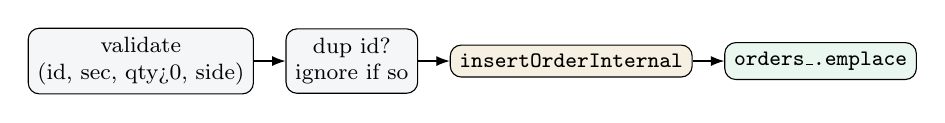
\begin{tikzpicture}[font=\footnotesize,>=Latex,node distance=4mm,every node/.style={align=center}]
  \node[draw,rounded corners,fill=Soft] (v) {validate\\(id, sec, qty>0, side)};
  \node[draw,rounded corners,fill=Soft,right=of v] (d) {dup id?\\ignore if so};
  \node[draw,rounded corners,fill=Gold!12,right=of d] (i) {\ttfamily insertOrderInternal};
  \node[draw,rounded corners,fill=Buy!10,right=of i] (s) {\ttfamily orders\_.emplace};
  \draw[->](v)--(d);\draw[->](d)--(i);\draw[->](i)--(s);
\end{tikzpicture}
\end{center}

\begin{lstlisting}
void OrderCache::addOrder(Order order) {
    if (!isValidOrder(order)) return;                      // reject garbage, no throw
    std::unique_lock<std::shared_mutex> lock(mutex_);      // WRITE lock
    if (orders_.count(order.orderId())) return;            // duplicate id: ignore
    insertOrderInternal(order);
    orders_.emplace(order.orderId(), std::move(order));    // truth updated last
}
\end{lstlisting}

\begin{pitfall}
State your policies: invalid orders and duplicate ids are \emph{silently ignored}
(not thrown). Trading systems prefer ``drop and continue'' to crashing. Both are
graded under ``robust error handling''.
\end{pitfall}

\subsection{\texttt{cancelOrder} --- handed an id}

\textbf{Handed:} just an id. \textbf{Forces:} nothing but a call to the helper ---
which already looks up by id and no-ops if absent.

\begin{lstlisting}
void OrderCache::cancelOrder(const std::string& orderId) {
    std::unique_lock<std::shared_mutex> lock(mutex_);
    removeOrderInternal(orderId);                          // unknown id -> no-op
}
\end{lstlisting}

\subsection{\texttt{cancelOrdersForUser} --- handed a user}

\textbf{Handed:} a user. \textbf{Forces:} start from the \emph{user index} to get
just that user's ids --- never scan all orders.

\begin{center}
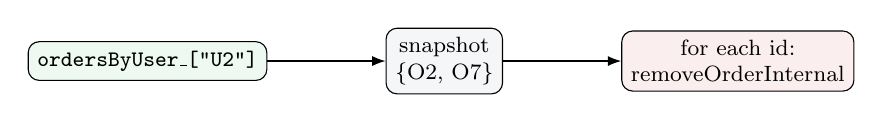
\begin{tikzpicture}[font=\footnotesize,>=Latex,every node/.style={align=center}]
  \node[draw,rounded corners,fill=Buy!8] (u) {\ttfamily ordersByUser\_["U2"]};
  \node[draw,rounded corners,fill=Soft,right=1.5cm of u] (list) {snapshot\\\{O2, O7\}};
  \node[draw,rounded corners,fill=Sell!8,right=1.5cm of list] (er) {for each id:\\removeOrderInternal};
  \draw[->](u)--(list);\draw[->](list)--(er);
\end{tikzpicture}
\end{center}

\begin{lstlisting}
void OrderCache::cancelOrdersForUser(const std::string& user) {
    std::unique_lock<std::shared_mutex> lock(mutex_);
    auto it = ordersByUser_.find(user);
    if (it == ordersByUser_.end()) return;
    // SNAPSHOT first: removeOrderInternal mutates ordersByUser_ as we go.
    const std::vector<std::string> ids(it->second.begin(), it->second.end());
    for (const std::string& id : ids) removeOrderInternal(id);
}
\end{lstlisting}

\begin{pitfall}
\textbf{Iterator invalidation.} \code{removeOrderInternal} erases from the very set
you'd loop over (and may erase the whole bucket). Iterating a container while
mutating it is undefined behavior. Copy the ids into a \code{vector} first, then
delete.
\end{pitfall}

\subsection{\texttt{cancelOrdersForSecIdWithMinimumQty} --- handed a security + threshold}

\textbf{Handed:} a security and a \code{minQty}. \textbf{Forces:} start from the
\emph{security index}, keep only ids with \code{qty >= minQty}, snapshot, delete.

\begin{lstlisting}
void OrderCache::cancelOrdersForSecIdWithMinimumQty(
        const std::string& securityId, unsigned int minQty) {
    std::unique_lock<std::shared_mutex> lock(mutex_);
    auto it = ordersBySecurity_.find(securityId);
    if (it == ordersBySecurity_.end()) return;
    std::vector<std::string> victims;                      // snapshot the matches
    for (const std::string& id : it->second) {
        auto o = orders_.find(id);
        if (o != orders_.end() && o->second.qty() >= minQty) victims.push_back(id);
    }
    for (const std::string& id : victims) removeOrderInternal(id);
}
\end{lstlisting}

\begin{pitfall}
The threshold is inclusive: \code{qty >= minQty}. An order whose qty \emph{equals}
\code{minQty} must be removed. Your test should assert \emph{which ids survive},
not just the count --- a \code{>} vs \code{>=} slip passes a count-only test.
\end{pitfall}

\subsection{\texttt{getMatchingSizeForSecurity} --- handed a security}

\textbf{Handed:} a security. \textbf{Forces:} read the maintained aggregate and
fold the \S3 formula over its companies. No order scan.

\begin{lstlisting}
unsigned int OrderCache::getMatchingSizeForSecurity(const std::string& securityId) {
    std::shared_lock<std::shared_mutex> lock(mutex_);      // READ lock (shared)
    auto it = securityTotals_.find(securityId);
    if (it == securityTotals_.end()) return 0;
    const SecurityTotals& agg = it->second;
    std::uint64_t reach = 0;                               // 64-bit: no overflow
    for (const auto& [company, ct] : agg.companies)
        reach += std::min<std::uint64_t>(ct.buy, agg.totalSell - ct.sell);
    std::uint64_t capped = std::min(reach, std::min(agg.totalBuy, agg.totalSell));
    return static_cast<unsigned int>(capped);              // header wants unsigned int
}
\end{lstlisting}

\subsection*{Aside --- what is a ``fold''? (for the layman)}
\addcontentsline{toc}{subsection}{\quad Aside: what is a fold}

I keep calling this method \emph{the fold}. Here is what that word means, because
it names the shape of the operation exactly.

A \textbf{fold} (also called \emph{reduce} or \emph{accumulate}) is the pattern of
\textbf{collapsing a whole collection down to a single value} by walking through it
and carrying a running result. The name is literal: like folding a long strip of
paper over and over until it is one small square, you take many items and fold
them into one.
\[
\text{fold:}\qquad [\,x_1,\ x_2,\ x_3,\ \dots,\ x_n\,]\ \longmapsto\ \text{one value}.
\]
Every fold has exactly three ingredients:

\begin{center}
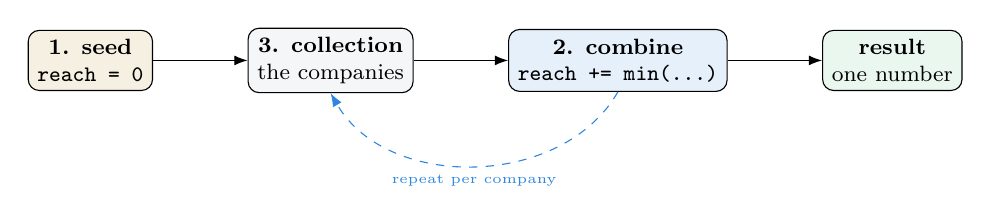
\begin{tikzpicture}[font=\footnotesize,>=Latex,node distance=6mm,every node/.style={align=center}]
  \node[draw,rounded corners,fill=Gold!12] (seed) {\textbf{1. seed}\\\ttfamily reach = 0};
  \node[draw,rounded corners,fill=Soft,right=1.2cm of seed] (coll) {\textbf{3. collection}\\the companies};
  \node[draw,rounded corners,fill=Accent!12,right=1.2cm of coll] (comb) {\textbf{2. combine}\\\ttfamily reach += min(\dots)};
  \node[draw,rounded corners,fill=Buy!10,right=1.2cm of comb] (out) {\textbf{result}\\one number};
  \draw[->](seed)--(coll);\draw[->](coll)--(comb);\draw[->](comb)--(out);
  \draw[->,dashed,Accent] (comb.south) to[out=-120,in=-60] node[below,font=\tiny]{repeat per company} (coll.south);
\end{tikzpicture}
\end{center}

Now map those onto the loop above:

\begin{center}
\renewcommand{\arraystretch}{1.3}\footnotesize
\begin{tabular}{@{}lll@{}}
\toprule
\textbf{Ingredient} & \textbf{In the code} & \\
\midrule
seed (starting value) & \ttfamily std::uint64\_t reach = 0; & \\
collection to walk & \ttfamily for (\dots : agg.companies) & \\
combine step & \ttfamily reach += min(ct.buy, totalSell - ct.sell); & \\
\bottomrule
\end{tabular}
\end{center}

That is precisely a fold: start at $0$, walk every company, accumulate each one's
contribution into the running \code{reach}. Many companies collapse into one
quantity.

\begin{intu}
In a language with folds built in you would write the \emph{same} operation as
\code{sum(min(c.buy, totalSell - c.sell) for c in companies)} (Python) or
\code{foldl' (\textbackslash acc c -> \dots) 0 companies} (Haskell). The C++
\code{for}-loop with a \code{+=} accumulator, the Python \code{sum}, and the
Haskell \code{foldl'} are all the \emph{same thing}. C++ even ships it by name:
\code{std::accumulate} \emph{is} the fold function --- our loop is just its
hand-written form.
\end{intu}

Why the word earns its place: it names the whole shape in one syllable, and it ties
back to the type-driven view (\S2) where matching's type is
$\ty{SecId}\to\ty{Qty}$ --- \emph{many in, one out}. A function that reduces a
structure to a summary value \emph{is} a fold (the fancy name is a
\emph{catamorphism}). It also sharply separates this method from its siblings:

\begin{center}
\renewcommand{\arraystretch}{1.25}\footnotesize
\begin{tabular}{@{}lll@{}}
\toprule
\textbf{Method} & \textbf{Shape} & \textbf{Name} \\
\midrule
\code{cancelOrder(id)} & key $\to$ find one thing & a \textbf{lookup} \\
\code{getAllOrders()} & structure $\to$ list of all & a \textbf{map / copy} \\
\code{getMatchingSizeForSecurity} & many companies $\to$ one number & a \textbf{fold} \\
\bottomrule
\end{tabular}
\end{center}

Only the matching query \emph{collapses many into one} --- which is why it, and
only it, is the fold.

\begin{pitfall}
Two traps. \textbf{(1)} Accumulate in \code{uint64\_t} and cast down only at the
end --- a million large-qty orders overflow 32 bits. \textbf{(2)}
\code{totalSell - ct.sell} can't underflow: a company's sells are always a subset
of the security's total sells (a maintained invariant).
\end{pitfall}

\subsection{\texttt{getAllOrders} --- handed nothing}

\textbf{Handed:} nothing. \textbf{Forces:} copy every value out of \code{orders\_}.
$O(n)$, and unavoidable --- you're returning all of it.

\begin{lstlisting}
std::vector<Order> OrderCache::getAllOrders() const {
    std::shared_lock<std::shared_mutex> lock(mutex_);
    std::vector<Order> out;
    out.reserve(orders_.size());
    for (const auto& [id, o] : orders_) out.push_back(o);
    return out;
}
\end{lstlisting}

\subsection{Locking, in one breath}

One \code{std::shared\_mutex}: the two \emph{reads} take a \code{shared\_lock}
(they run concurrently); the four \emph{writes} take a \code{unique\_lock}. The
aggregate is always consistent with \code{orders\_} because both change under the
same write lock. Mention it; don't over-build it.

\begin{say}
``Each method starts from the structure keyed by what it's handed --- id, user,
security, or nothing. The three cancels all funnel into one
\code{removeOrderInternal}, so the four structures stay in sync from a single
place, and bulk cancels snapshot ids first to dodge iterator invalidation.
Matching reads the aggregate as an $O(\#\text{companies})$ 64-bit fold. Reads take
a shared lock, writes a unique lock.''
\end{say}

\clearpage
\section{The reference implementation, taught line by line}

Now we assemble the actual C++ --- pragmatic, type-aware, \emph{not}
over-engineered. We build it in the order you'd write it live, explaining the
\emph{why} behind every decision so you can reproduce it from understanding, not
memory. Target: clean C++17 that compiles, with the aggregate design from \S5.

\subsection{Design contract (say this first, before typing)}

\begin{keybox}[The one-paragraph design you announce]
``The cache is a tiny in-memory database: one hash map \code{orders\_} as the
single source of truth, two secondary indexes (\code{ordersByUser\_},
\code{ordersBySecurity\_}) for targeted cancels, and a per-security
\code{aggregate} that acts as a materialized view so matching is a fast fold.
Every write updates all four through two private helpers, so the indexes can
never desync. Matching uses the per-company formula, not naive $\min$.''
\end{keybox}

\subsection{Writing the header (\texttt{.hpp}) from first principles}

You don't memorise the header --- you \emph{derive} it by asking three questions.

\textbf{Q1. What must each operation look up quickly?} That decides the member
maps. \code{cancelOrder} gets an \emph{id} $\Rightarrow$ a map from id. The two
bulk cancels get a \emph{user} / \emph{security} $\Rightarrow$ a map from each:

\begin{lstlisting}
// the ONE owner of order data; find any order by id in O(1)
std::unordered_map<std::string, Order> orders_;
// index: user -> that user's order ids  (cancelForUser touches only these)
std::unordered_map<std::string, std::unordered_set<std::string>> ordersByUser_;
// index: security -> that security's order ids
std::unordered_map<std::string, std::unordered_set<std::string>> ordersBySecurity_;
\end{lstlisting}

\textbf{Q2. What does the matching \emph{formula} need?} It reads, per security,
the total sell $S$ and each company's $b_c,s_c$. So build a struct that \emph{is}
those inputs, pre-summed --- nothing more:

\begin{lstlisting}
struct CompanyTotals  { std::uint64_t buy = 0, sell = 0; };   // one firm's b_c, s_c
struct SecurityTotals {
    std::uint64_t totalBuy = 0, totalSell = 0;                // B and S
    std::unordered_map<std::string, CompanyTotals> companies; // per-company b_c,s_c
};
std::unordered_map<std::string, SecurityTotals> securityTotals_;   // secId -> aggregate
\end{lstlisting}

\begin{intu}
Map the struct onto the formula so it stops being abstract: \code{totalSell} is
the $S$ in $S-s_c$; \code{companies["A"].buy} is $b_A$; \code{companies["A"].sell}
is $s_A$. The struct is \emph{literally the numbers the fold will read} --- you
store exactly what $\sum_c\min(b_c,\,S-s_c)$ needs, so the query never touches an
individual order.
\end{intu}

\textbf{Q3. What keeps the four structures consistent?} Two private helpers (so
there is one place to get it right) plus the lock:

\begin{lstlisting}
private:
    static bool isValidOrder(const Order& order);          // reject garbage
    void insertOrderInternal(const Order& order);          // add to all 4
    bool removeOrderInternal(const std::string& orderId);  // remove from all 4
    mutable std::shared_mutex mutex_;                       // reads share, writes exclude
\end{lstlisting}

That is the entire header logic: \textbf{truth map $+$ two indexes $+$ one
aggregate $+$ two helpers $+$ a lock}. The six public methods are just
\code{override} declarations of the fixed interface signatures.

\subsection{Types: normalize \texttt{Side} at the boundary}

The header forces \code{side} to be a \code{std::string} (we can't change
\code{Order}). But \emph{internally} we treat it as a two-value domain --- this is
the ``make illegal states unrepresentable'' idea, applied pragmatically at the
edge:

\begin{lstlisting}
namespace {
enum class Side { Buy, Sell };

// Parse the accepted spellings once, at the door. Anything else is invalid.
bool parseSide(const std::string& s, Side& out) {
    if (s == "Buy"  || s == "buy"  || s == "BUY")  { out = Side::Buy;  return true; }
    if (s == "Sell" || s == "sell" || s == "SELL") { out = Side::Sell; return true; }
    return false;                     // unknown side -> reject the order
}
}  // namespace
\end{lstlisting}

\begin{intu}
We don't rewrite \code{Order} (the spec forbids it), so we \emph{convert} the
string to a clean enum \textbf{once}, right where data enters the system. After
that boundary, no code branches on raw strings --- the whole class of ``what if
side is \code{"xyz"}?'' bugs is gone because such an order never gets stored.
\end{intu}

\subsection{Validation: reject garbage at the door}

The prompt grades ``robust error handling.'' One small helper, called first in
\code{addOrder}:

\begin{lstlisting}
static bool isValidOrder(const Order& o) {
    if (o.orderId().empty())    return false;   // ids must exist
    if (o.securityId().empty()) return false;
    if (o.qty() == 0)           return false;   // a zero-qty order is meaningless
    Side tmp;
    if (!parseSide(o.side(), tmp)) return false;// side must be Buy/Sell
    return true;                                // user/company may be empty by spec
}
\end{lstlisting}

\begin{pitfall}
Decide your policy and \emph{state} it: invalid orders are \textbf{silently
ignored} (not thrown). Trading systems prefer ``drop and continue'' over crashing
the process. Same for duplicate ids and unknown-id cancels --- graceful no-ops.
\end{pitfall}

\subsection{The two sync helpers (invariants live in exactly one place)}

Every structure is touched only through these. Write them once, reuse everywhere.

\begin{lstlisting}
// Add an already-validated order to indexes + aggregate. (side already parsed.)
void OrderCache::addToTotals(const Order& o, Side side) {
    auto& agg = securityTotals_[o.securityId()];
    auto& co  = agg.companies[o.company()];
    if (side == Side::Buy) { agg.totalBuy  += o.qty(); co.buy  += o.qty(); }
    else                   { agg.totalSell += o.qty(); co.sell += o.qty(); }
}

// Remove an order from ALL four structures by id. Returns false if absent.
bool OrderCache::removeOrderInternal(const std::string& id) {
    auto it = orders_.find(id);
    if (it == orders_.end()) return false;      // unknown id: graceful no-op
    const Order o = it->second;                 // copy: we erase the map entry below

    // 1) user index -- drop the bucket when it empties so maps don't grow forever
    if (auto u = ordersByUser_.find(o.user()); u != ordersByUser_.end()) {
        u->second.erase(id);
        if (u->second.empty()) ordersByUser_.erase(u);
    }
    // 2) security index
    if (auto s = ordersBySecurity_.find(o.securityId()); s != ordersBySecurity_.end()) {
        s->second.erase(id);
        if (s->second.empty()) ordersBySecurity_.erase(s);
    }
    // 3) aggregate -- subtract this order's contribution, prune zeros
    if (auto a = securityTotals_.find(o.securityId()); a != securityTotals_.end()) {
        Side side; parseSide(o.side(), side);   // valid: it was validated on insert
        auto& agg = a->second;
        auto  c   = agg.companies.find(o.company());
        if (c != agg.companies.end()) {
            if (side == Side::Buy) { agg.totalBuy  -= o.qty(); c->second.buy  -= o.qty(); }
            else                   { agg.totalSell -= o.qty(); c->second.sell -= o.qty(); }
            if (c->second.buy == 0 && c->second.sell == 0) agg.companies.erase(c);
        }
        if (agg.companies.empty()) securityTotals_.erase(a);
    }
    // 4) source of truth -- last, since we needed o above
    orders_.erase(it);
    return true;
}
\end{lstlisting}

\begin{intu}
Notice the discipline: \emph{copy} the order out before erasing, prune empty
buckets so memory doesn't leak, and touch \code{orders\_} \emph{last}. Every
cancel path in the class routes through this one function --- so there is exactly
one place that can get invariant maintenance wrong, and it's under your eye.
\end{intu}

\subsection{\texttt{addOrder} --- validate, dedup, store, index}

\begin{lstlisting}
void OrderCache::addOrder(Order order) {
    if (!isValidOrder(order)) return;                 // graceful reject
    std::unique_lock lock(mutex_);                    // WRITE lock
    if (orders_.count(order.orderId())) return;       // duplicate id: ignore

    Side side; parseSide(order.side(), side);         // guaranteed to succeed now
    ordersByUser_[order.user()].insert(order.orderId());
    ordersBySecurity_[order.securityId()].insert(order.orderId());
    addToTotals(order, side);
    orders_.emplace(order.orderId(), std::move(order));
}
\end{lstlisting}

\subsection{The three cancels --- all built on \texttt{removeOrderInternal}}

\begin{lstlisting}
void OrderCache::cancelOrder(const std::string& orderId) {
    std::unique_lock lock(mutex_);
    removeOrderInternal(orderId);                     // absent id -> no-op
}

void OrderCache::cancelOrdersForUser(const std::string& user) {
    std::unique_lock lock(mutex_);
    auto it = ordersByUser_.find(user);
    if (it == ordersByUser_.end()) return;
    // SNAPSHOT ids first -- removeOrderInternal mutates ordersByUser_ as we go.
    std::vector<std::string> ids(it->second.begin(), it->second.end());
    for (const auto& id : ids) removeOrderInternal(id);
}

void OrderCache::cancelOrdersForSecIdWithMinimumQty(
        const std::string& securityId, unsigned int minQty) {
    std::unique_lock lock(mutex_);
    auto it = ordersBySecurity_.find(securityId);
    if (it == ordersBySecurity_.end()) return;
    std::vector<std::string> victims;                 // snapshot the ones to kill
    for (const auto& id : it->second) {
        auto o = orders_.find(id);
        if (o != orders_.end() && o->second.qty() >= minQty) victims.push_back(id);
    }
    for (const auto& id : victims) removeOrderInternal(id);
}
\end{lstlisting}

\begin{pitfall}
\textbf{Iterator invalidation} is the trap here. \code{removeOrderInternal}
erases from the very set you'd be looping over. So we copy the ids into a
\code{vector} \emph{first}, then delete. Looping a container while mutating it is
undefined behavior --- snapshot, then act.
\end{pitfall}

\subsection{\texttt{getMatchingSizeForSecurity} --- the fold}

\begin{lstlisting}
unsigned int OrderCache::getMatchingSizeForSecurity(const std::string& securityId) {
    std::shared_lock lock(mutex_);                    // READ lock (shared)
    auto it = securityTotals_.find(securityId);
    if (it == securityTotals_.end()) return 0;
    const SecurityTotals& agg = it->second;

    // per-company reach: each company's buys matched vs everyone ELSE's sells
    std::uint64_t reach = 0;                           // 64-bit: avoid overflow
    for (const auto& [company, ct] : agg.companies)
        reach += std::min<std::uint64_t>(ct.buy, agg.totalSell - ct.sell);

    std::uint64_t capped = std::min(reach, std::min(agg.totalBuy, agg.totalSell));
    return static_cast<unsigned int>(capped);          // header demands unsigned int
}
\end{lstlisting}

\begin{pitfall}
Two subtleties. \textbf{(1)} Accumulate in \code{uint64\_t} --- a million orders
of large \code{qty} overflow 32 bits; only cast down at the very end. \textbf{(2)}
\code{totalSell - ct.sell} is safe because a company's sells never exceed the
security's total sells (invariant), so it can't underflow.
\end{pitfall}

\subsection{\texttt{getAllOrders} --- the dump}

\begin{lstlisting}
std::vector<Order> OrderCache::getAllOrders() const {
    std::shared_lock lock(mutex_);
    std::vector<Order> out;
    out.reserve(orders_.size());
    for (const auto& [id, o] : orders_) out.push_back(o);
    return out;
}
\end{lstlisting}

\subsection{Header additions you'd declare}

Add the two private helpers and forward-declare \code{Side} usage. Since
\code{Side} is a file-local enum in the \code{.cpp}, the helper takes it there;
in the header we only declare:

\begin{lstlisting}
private:
    static bool isValidOrder(const Order& order);
    bool removeOrderInternal(const std::string& orderId);
    // addToTotals is a .cpp detail; if declared in the header, take an int/bool
    // "isBuy" instead of the file-local Side enum to keep the header clean.
\end{lstlisting}

\begin{keybox}[Why this is ``type-driven but not over-engineered'']
We used types where they \emph{earn their keep}: a two-value \code{Side} enum at
the boundary (illegal sides unrepresentable), a small \code{struct} aggregate
(exactly the state the fold needs), \code{std::optional} for parsing, and
\code{uint64\_t} accumulators (the right numeric domain). We \emph{avoided}
gold-plating: no max-flow engine, no template metaprogramming, no premature
sharding --- just the closed-form fold over a maintained aggregate. That balance
is the senior signal.
\end{keybox}

\begin{pitfall}[\faBalanceScale~What to deliberately NOT do (the restraint signal)]
A take-home is graded on judgment, and \textbf{knowing where to stop} is half of
it. State these choices in your \code{DESIGN.md} explicitly:
\begin{itemize}[leftmargin=1.3em,nosep]
  \item \textbf{No max-flow solver} --- the per-company sum is provably optimal, so
        a flow engine is more code for the same answer.
  \item \textbf{No strong typedefs for every id field} --- the frozen \code{Order}
        returns \code{std::string}, so tagged ids force conversions everywhere for
        marginal benefit.
  \item \textbf{No \code{Validated<Order>} phantom wrapper} --- elegant, but pure
        plumbing that doesn't change what's graded.
  \item \textbf{No sharding / lock-free} --- one \code{shared\_mutex} is correct
        and simple; shard by \code{securityId} \emph{only} if profiling shows
        contention.
\end{itemize}
Writing the ``what I did not do and why'' paragraph is itself a seniority signal:
it shows you saw the fancy options and \emph{chose} the proportionate one.
\end{pitfall}

\begin{keybox}[This code is real and verified]
The listings above are the actual delivered files, not pseudocode. They compile
clean under \code{g++ -std=c++17 -Wall -Wextra} (zero warnings), pass a
\textbf{16-test} suite (including a 5000-case property test vs.\ an independent
oracle and a million-order timing test), and run clean under
\code{-fsanitize=address,undefined}. See the \code{solution/} folder next to this
PDF and \code{DESIGN.md} for the full write-up.
\end{keybox}

\begin{say}
``I normalize side to an enum at the boundary so illegal states can't be stored,
validate and reject garbage gracefully, and funnel every mutation through two
helpers so the source of truth, two indexes, and the per-security aggregate stay
in lockstep. Cancels snapshot ids before deleting to dodge iterator
invalidation. Matching is a 64-bit fold over the aggregate in $O(\#\text{companies})$,
cast to \code{unsigned int} at the end. Reads take a shared lock, writes a unique
lock.''
\end{say}

\clearpage
\section{How to think about testing (from zero)}

Most people write tests by listing cases they happen to think of. That is layer-1
thinking and it gives false confidence. This section teaches the \emph{mental
models} that let you \emph{generate} tests systematically --- so you could build a
convincing suite for \emph{any} problem, and defend every test you wrote. The
concrete GoogleTest code follows in the next two sections; here we build the
\emph{judgment}.

\subsection{The core idea: a test is a trap for a specific bug}

A good test is not ``check it works.'' It is \textbf{a trap set for one particular
way the code could be wrong.} Before writing a test, finish this sentence:
\emph{``This test fails if the code \dots''}. If you can't name the bug, the test
isn't earning its place.

\begin{keybox}[The proof that weak tests lie]
Take a \emph{wrong} matching implementation --- the naive $\min(\text{buy},\text{sell})$
that ignores the company rule. Run it against ``obvious'' tests:
\begin{center}\footnotesize
\begin{tabular}{@{}lccc@{}}
\toprule
test & correct & naive-wrong & naive passes? \\
\midrule
partial (Buy 100 A, Sell 300 B) & $100$ & $100$ & \textcolor{Sell}{\textbf{yes}} \\
only buys & $0$ & $0$ & \textcolor{Sell}{\textbf{yes}} \\
simple cross & $100$ & $100$ & \textcolor{Sell}{\textbf{yes}} \\
self-only (Buy 100 A, Sell 100 A) & $0$ & $100$ & \textcolor{Buy}{no} \\
\textbf{dominant company} & $150$ & $950$ & \textcolor{Buy}{no} \\
\bottomrule
\end{tabular}
\end{center}
The broken code \textbf{passes three of five ``obvious'' tests.} Only the two tests
\emph{designed to discriminate} catch it. \emph{A suite that doesn't distinguish
right from a plausible wrong is theatre.}
\end{keybox}

\subsection{Mental model 1 --- read the tests off the formula}

Every term in a formula is a place the code can go wrong, so every term suggests a
test. Look at $M=\min(B,\ S,\ B+S-\max_c(b_c+s_c))$:

\begin{center}
\renewcommand{\arraystretch}{1.3}\footnotesize
\begin{tabular}{@{}p{3.2cm}p{5.3cm}p{5.0cm}@{}}
\toprule
\textbf{Term} & \textbf{Test that pins it} & \textbf{Fails if\dots} \\
\midrule
the $B$ (buy cap) & buys $<$ sells, cross-company & you cap by the wrong side \\
the $S$ (sell cap) & sells $<$ buys, cross-company & same, other side \\
the $-\max_c(\dots)$ term & \textbf{dominant company} & you used naive $\min$ \\
the different-company rule & self-only $\to 0$ & you match a firm with itself \\
\bottomrule
\end{tabular}
\end{center}

\begin{intu}
This is why the dominant-company test is \emph{the} test: it is the only one that
exercises the third, non-obvious term. If your suite has no test where one company
holds a big chunk of both sides, you have not tested the actual hard part.
\end{intu}

\subsection{Mental model 2 --- test at the boundaries, not the middle}

Bugs hide at edges, not in the comfortable interior. For every quantity, ask
``what are its extremes?'' and test each:

\begin{itemize}[leftmargin=1.5em,nosep]
  \item \textbf{Empty} --- no orders, unknown security/user/id. (Does it crash or
        return $0$/empty gracefully?)
  \item \textbf{One} --- a single order, a single company. (One company $\to$ always $0$.)
  \item \textbf{The threshold itself} --- \code{minQty} exactly equal to an order's
        qty. (\code{>} vs \code{>=} off-by-one.)
  \item \textbf{Huge} --- quantities near the type's max. (32-bit overflow.)
  \item \textbf{Duplicate} --- same id added twice. (Which policy fires?)
\end{itemize}

\begin{intu}
``Off-by-one'' and ``forgot the empty case'' are the two most common bugs in all
of software. Boundary tests are how you catch them on purpose instead of in
production. When you see \code{>=} in the code, you should reflexively write the
$=$ case.
\end{intu}

\subsection{Mental model 3 --- test relationships, not just values}

Fixed-value tests (``input $X$ gives $42$'') only cover cases you computed by hand.
\textbf{Metamorphic} tests check a \emph{relationship} that must hold for
\emph{every} input --- so they cover infinitely many cases you never enumerated.

\begin{center}
\renewcommand{\arraystretch}{1.3}\footnotesize
\begin{tabular}{@{}p{5.0cm}p{8.3cm}@{}}
\toprule
\textbf{Relationship (must always hold)} & \textbf{The bug it catches} \\
\midrule
add $X$ then cancel $X$ $\Rightarrow$ back to start & aggregate updated on add but not on cancel \\
insertion order doesn't change matching & hidden order-dependent state \\
cancel-for-user $\Rightarrow$ none of that user's orders remain & index desync / leftover ghosts \\
matching $\le \min(B,S)$ always & the cap logic is wrong \\
\bottomrule
\end{tabular}
\end{center}

\begin{intu}
The \emph{add-then-cancel round trip} is the single most valuable consistency test
here, because the \#1 bug in this design is ``I decrement the aggregate wrong on
cancel.'' If add-then-cancel returns you to the exact starting numbers, your two
sync helpers are mirror images --- which is the whole correctness argument.
\end{intu}

\subsection{Mental model 4 --- the oracle (test against a second brain)}

The most powerful idea in testing: compute the answer \textbf{two different ways}
and demand they agree. The second way --- the \textbf{oracle} --- must be written
\emph{differently} so it can't share a bug with the first.

\begin{center}
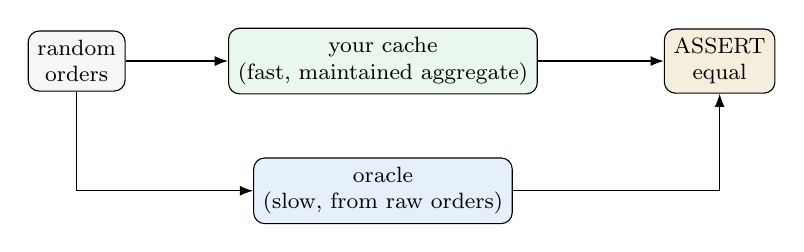
\begin{tikzpicture}[font=\footnotesize,>=Latex,node distance=8mm,every node/.style={align=center}]
  \node[draw,rounded corners,fill=Soft] (g) {random\\orders};
  \node[draw,rounded corners,fill=Buy!10,right=1.3cm of g] (i) {your cache\\(fast, maintained aggregate)};
  \node[draw,rounded corners,fill=Accent!12,below=8mm of i] (o) {oracle\\(slow, from raw orders)};
  \node[draw,rounded corners,fill=Gold!14,right=1.6cm of i] (c) {ASSERT\\equal};
  \draw[->](g)--(i); \draw[->](g)|-(o); \draw[->](i)--(c); \draw[->](o)-|(c);
\end{tikzpicture}
\end{center}

\begin{intu}
Why does this work? A bug in your fast code is unlikely to be \emph{the same} bug
in a slow, independently-written reference. So when they disagree on some random
input, one of them is wrong --- and you've found a case you'd never have dreamed up
by hand. Run it on thousands of random inputs (with a \textbf{fixed seed} so
failures reproduce) and you've effectively tested the space, not a handful of
points.
\end{intu}

\begin{pitfall}
The oracle must be \emph{obviously correct} and \emph{independent}. A subtle trap
here: a naive $O(n^2)$ greedy pairing is \emph{not} a correct oracle (greedy
under-counts, \S on math). The safe oracle is the per-company formula recomputed
from the \emph{raw order list} --- it re-derives the answer without reusing the
cache's maintained aggregate, so it catches maintenance bugs, which are the likely
ones.
\end{pitfall}

\subsection{Mental model 5 --- test the \emph{promise}, not just correctness}

The spec promised efficiency at a million orders. That is a claim your tests should
\emph{enforce}, because a correct-but-slow implementation (one that scans all orders
per query) passes every correctness test and still fails the real requirement.

\begin{intu}
A performance test is a correctness test for your \emph{design}. Insert a million
orders, time one \code{getMatchingSizeForSecurity}, assert it's under a few
milliseconds. A scanning implementation blows the budget; your aggregate
implementation sails through. The test is what proves the design paid off.
\end{intu}

\subsection{Putting the layers together (the pyramid)}

\begin{center}
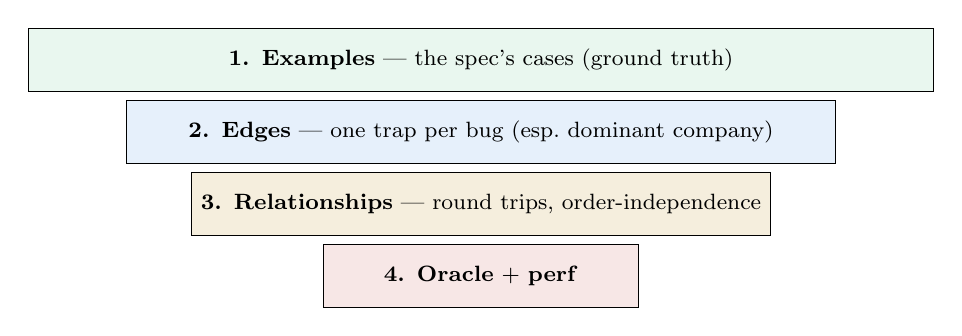
\begin{tikzpicture}[font=\footnotesize]
  \node[draw,fill=Buy!10,minimum width=11.5cm,minimum height=0.8cm] (l1){\textbf{1. Examples} --- the spec's cases (ground truth)};
  \node[draw,fill=Accent!12,minimum width=9cm,minimum height=0.8cm,below=1mm of l1] (l2){\textbf{2. Edges} --- one trap per bug (esp.\ dominant company)};
  \node[draw,fill=Gold!14,minimum width=6.5cm,minimum height=0.8cm,below=1mm of l2] (l3){\textbf{3. Relationships} --- round trips, order-independence};
  \node[draw,fill=Sell!12,minimum width=4cm,minimum height=0.8cm,below=1mm of l3] (l4){\textbf{4. Oracle} + \textbf{perf}};
\end{tikzpicture}
\end{center}

\noindent Bottom-up: examples prove it works on known cases; edges catch the
specific bugs; relationships cover the unenumerated cases; the oracle covers the
\emph{space}; the perf test enforces the promise. A suite with all four reads as
\emph{engineering}, not homework --- which is exactly what a take-home grades.

\begin{say}
``I think of each test as a trap for one bug. I read the edge cases off the
formula --- the dominant-company case is the one that separates correct from naive.
I add relationship tests like add/cancel round-trips that catch aggregate-desync,
and a property test against an independent oracle on thousands of fixed-seed random
inputs so I'm testing the space, not points. Finally a million-order timing test
enforces the efficiency promise. I run it all under sanitizers so overflow and
iterator bugs fail loudly.''
\end{say}

\subsection{Blank-page drill --- generate the whole suite cold}

The real skill is producing the suite from \emph{nothing}. Close the document. On
a blank page, for each of the six methods, write every test you'd add \textbf{and
the one-line bug it traps}. Then uncover the checklist below and score yourself.

\begin{keybox}[Target: name the test \emph{and} the bug it catches]
\footnotesize
\renewcommand{\arraystretch}{1.25}
\begin{tabular}{@{}p{5.6cm}p{7.4cm}@{}}
\toprule
\textbf{Test you should recall} & \textbf{Bug it traps (say this too)} \\
\midrule
\multicolumn{2}{@{}l}{\textit{\color{Accent}Layer 1 --- examples}}\\
README example ($2700$) & baseline: the formula is plain wrong \\[2pt]
\multicolumn{2}{@{}l}{\textit{\color{Accent}Layer 2 --- edges (one trap each)}}\\
self-only $\to 0$ & a firm matches with itself \\
one cross-company match & counting own-company sells \\
\textbf{dominant company} $\to 150$ & using naive $\min(B,S)$ \\
only-one-side $\to 0$ & missing the empty-side guard \\
invalid orders ignored & no validation (empty id, qty 0, bad side) \\
duplicate id ignored & second add overwrites / corrupts \\
unknown lookup/cancel = no-op & missing graceful guard (throws) \\
\code{minQty} boundary ($=$) survives-check & \code{>} vs \code{>=} off-by-one \\
overflow (near \code{UINT\_MAX}) & 32-bit accumulator \\[2pt]
\multicolumn{2}{@{}l}{\textit{\color{Accent}Layer 3 --- relationships}}\\
add $\to$ cancel restores matching & aggregate not decremented on cancel \\
cancel-for-user leaves no trace & index desync / ghost ids \\
insertion order irrelevant & hidden order-dependent state \\[2pt]
\multicolumn{2}{@{}l}{\textit{\color{Accent}Layer 4 --- oracle + promise}}\\
random vs.\ oracle (fixed seed) & any matching bug, on cases you'd never dream up \\
random add/cancel vs.\ oracle & maintenance bug under churn \\
million-order timing & an $O(n)$ scan sneaking into the query \\
\bottomrule
\end{tabular}
\end{keybox}

\textbf{Score yourself:}
\begin{itemize}[leftmargin=1.5em,nosep]
  \item \textbf{$<8$ recalled} --- you're listing cases, not thinking in layers.
        Re-read the five mental models; the goal is to \emph{derive} these, not
        memorize them.
  \item \textbf{8--13} --- solid. Note \emph{which layer} you dropped (usually 3
        or 4 --- everyone remembers examples and edges).
  \item \textbf{14+} with the bug named for each --- you can defend a suite in the
        interview. Re-blank-page it tomorrow to make it permanent.
\end{itemize}

\begin{intu}
The trick to never blanking: don't memorize the 16 rows --- memorize the
\textbf{four layers} and the \textbf{five mental models}, then regenerate the rows
from them. ``Read tests off the formula'' alone gives you the whole edge layer;
``test relationships'' gives you layer 3; ``oracle + promise'' gives you layer 4.
The list is downstream of the thinking.
\end{intu}

\clearpage
\section{Testing, done properly}

The prompt says plainly: \emph{``The quality of your test suite is part of the
evaluation \dots\ we are looking for evidence of thoughtful test design.''} That
means tests are graded like production code. This section gives you a
\emph{theory} of how to test this problem, not just a list --- so you can justify
every test and add the ones most candidates forget: an \textbf{oracle}, a
\textbf{property-based} layer, \textbf{consistency} tests, and a
\textbf{performance} test.

\subsection{The four layers of a convincing suite}

\begin{center}
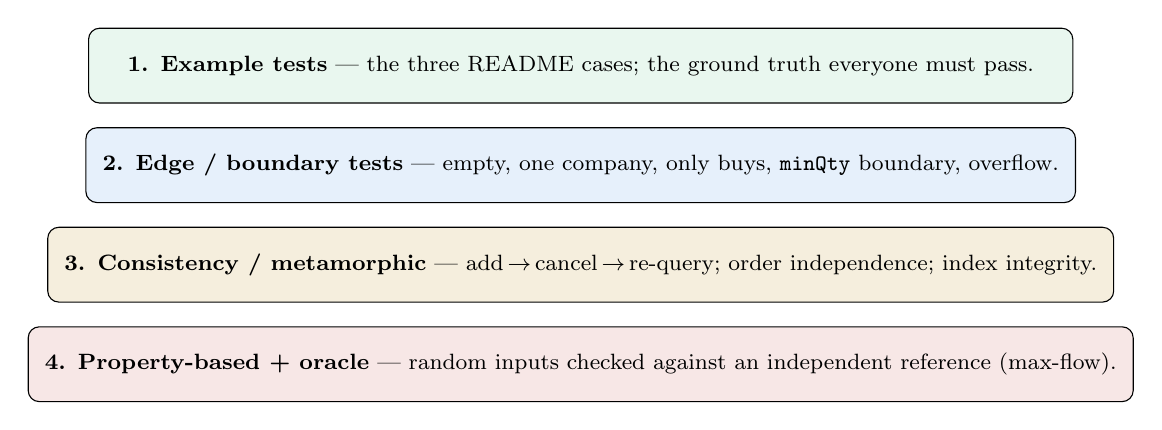
\begin{tikzpicture}[font=\footnotesize,>=Latex]
  \tikzstyle{lay}=[draw,rounded corners,minimum width=12.5cm,minimum height=0.95cm,align=left,inner sep=6pt]
  \node[lay,fill=Buy!10] (l1) {\textbf{1. Example tests} --- the three README cases; the ground truth everyone must pass.};
  \node[lay,fill=Accent!12,below=3mm of l1] (l2) {\textbf{2. Edge / boundary tests} --- empty, one company, only buys, \texttt{minQty} boundary, overflow.};
  \node[lay,fill=Gold!14,below=3mm of l2] (l3) {\textbf{3. Consistency / metamorphic} --- add\,$\to$\,cancel\,$\to$\,re-query; order independence; index integrity.};
  \node[lay,fill=Sell!12,below=3mm of l3] (l4) {\textbf{4. Property-based + oracle} --- random inputs checked against an independent reference (max-flow).};
\end{tikzpicture}
\end{center}

\begin{intu}
Layers 1--2 prove ``it works on the cases I \emph{thought} of''. Layers 3--4 prove
``it works on cases I did \emph{not} think of'' --- which is the whole point of
testing. Interviewers notice immediately when you climb past layer 2, because
almost nobody does.
\end{intu}

\subsection{Layer 1 --- the example tests (necessary, not sufficient)}

The three README examples ($2700$, and the Example~2 / Example~3 tables) are
non-negotiable. Your starter suite already has them, e.g.:

\begin{lstlisting}
EXPECT_EQ(cache.getMatchingSizeForSecurity("SecId2"), 2700);
EXPECT_EQ(cache.getMatchingSizeForSecurity("SecId1"), 0);   // same-company
EXPECT_EQ(cache.getMatchingSizeForSecurity("SecId3"), 0);   // only buys
\end{lstlisting}

\begin{pitfall}
Passing the three examples proves \emph{almost nothing} on its own --- a wrong
\code{min(B,S)} implementation passes two of the three SecIds in Example~1! You
must add cases that \emph{distinguish} the right formula from the plausible wrong
ones. That is what the next layers are for.
\end{pitfall}

\subsection{Layer 2 --- edges chosen to kill specific bugs}

Every edge case should be traceable to a bug it would catch. Design them from the
formula $M=\min(B,S,\,B+S-\max_c(b_c+s_c))$: each term suggests a test.

\begin{center}
\renewcommand{\arraystretch}{1.3}\footnotesize
\begin{tabular}{@{}p{4.3cm}p{5.5cm}p{4.0cm}@{}}
\toprule
\textbf{Test} & \textbf{Input} & \textbf{Catches} \\
\midrule
one company only & \Buy{}500(A), \Sell{}500(A) $\to$ \textbf{0} & forgetting the company rule \\
one cross match & \Buy{}100(A), \Sell{}100(A), \Sell{}100(B) $\to$ \textbf{100} & counting own-company sells \\
\textbf{dominant company} & \Buy{}1000(A), \Sell{}900(A), \Buy{}100(B), \Sell{}50(C) $\to$ \textbf{150} & using naive $\min(B,S){=}950$ \\
only buys / only sells & all one side $\to$ \textbf{0} & missing empty-side guard \\
partial match & \Buy{}100, \Sell{}300 (diff co) $\to$ \textbf{100} & wrong side cap \\
\code{minQty} boundary & cancel with qty \emph{exactly} $=$ minQty & \code{>} vs \code{>=} off-by-one \\
unknown security / id / user & any lookup $\to$ no-op, no throw & missing graceful guard \\
overflow & many orders of qty near \code{UINT\_MAX} & 32-bit accumulator \\
\bottomrule
\end{tabular}
\end{center}

\begin{keybox}[The star edge case: dominant company]
\Buy{}1000(A), \Sell{}900(A), \Buy{}100(B), \Sell{}50(C). Here $B{=}1100$,
$S{=}950$, so a naive implementation returns $\min(1100,950){=}\mathbf{950}$. The
\emph{correct} answer is $\mathbf{150}$ (company A's huge position can only trade
with B and C's tiny opposite side). This single test separates a correct solution
from the most common wrong one. Put it in your suite and \emph{mention it}.
\end{keybox}

\subsection{Layer 3 --- consistency and metamorphic tests}

These check \emph{relationships} between operations rather than fixed answers.
They are cheap to write and catch the desync bugs from \S5.

\begin{itemize}[leftmargin=1.5em]
  \item \textbf{Add--cancel round trip.} After \code{addOrder} then
        \code{cancelOrder} of the same id, the cache must be byte-for-byte back to
        its earlier state: same \code{getAllOrders} size, \emph{and} same matching
        numbers. This catches aggregates that are updated on add but not on cancel.
  \item \textbf{Order independence (commutativity).} Insert the same orders in a
        different order; every \code{getMatchingSizeForSecurity} must be identical.
        Verified true in theory (matching depends only on the multiset of orders).
        A failure means hidden order-dependent state. \emph{(0 violations across
        50{,}000 random shuffles in my check.)}
  \item \textbf{Self-pair monotonicity (metamorphic).} Adding a brand-new
        company's matching buy+sell pair can never \emph{decrease} any security's
        match size. \emph{(0 violations in 50{,}000 trials.)}
  \item \textbf{Index integrity after bulk cancels.} After
        \code{cancelOrdersForUser}, no leftover order in \code{getAllOrders}
        belongs to that user, and querying that user again is a clean no-op.
\end{itemize}

\begin{lstlisting}
TEST_F(OrderCacheTest, AddCancelRoundTripRestoresMatching) {
    seedExample1(cache);                       // some fixed scenario
    auto before = cache.getMatchingSizeForSecurity("SecId2");
    cache.addOrder({"TMP","SecId2","Sell",123,"UX","CompZ"});
    cache.cancelOrder("TMP");
    EXPECT_EQ(cache.getMatchingSizeForSecurity("SecId2"), before); // aggregate healed
}
\end{lstlisting}

\subsection{Layer 4 --- property-based testing with an oracle}

This is the layer that turns ``I hope it's right'' into ``I \emph{proved} it's
right on 100k cases''. The idea, from QuickCheck-style testing:

\begin{center}
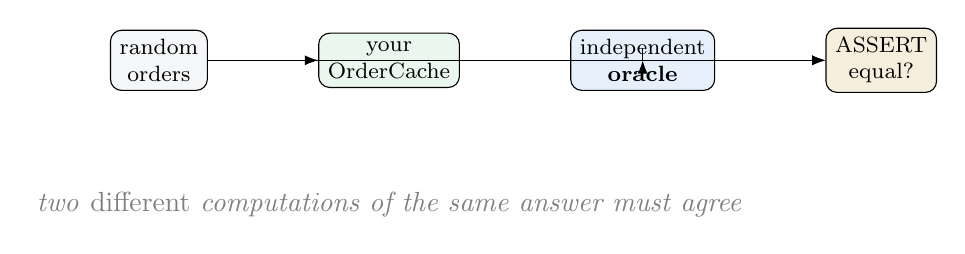
\begin{tikzpicture}[font=\footnotesize,>=Latex,node distance=8mm,every node/.style={align=center}]
  \node[draw,rounded corners,fill=Soft] (gen) {random\\orders};
  \node[draw,rounded corners,fill=Buy!10,right=1.4cm of gen] (impl) {your\\OrderCache};
  \node[draw,rounded corners,fill=Accent!12,right=1.4cm of impl] (orc) {independent\\\textbf{oracle}};
  \node[draw,rounded corners,fill=Gold!14,right=1.4cm of orc] (cmp) {ASSERT\\equal?};
  \draw[->](gen)--(impl);\draw[->](gen)-|(orc);\draw[->](impl)--(cmp);\draw[->](orc)|-(cmp);
  \node[below=1.2cm of impl,align=center,font=\itshape\color{gray}]
    {two \emph{different} computations of the same answer must agree};
\end{tikzpicture}
\end{center}

The oracle must be written a \emph{different way} than the implementation so they
don't share a bug. Two good oracles here:

\begin{enumerate}[leftmargin=1.5em]
  \item \textbf{Brute max-flow} (Edmonds--Karp on the tiny company graph). This is
        the gold standard --- it computes the true optimum from first principles.
        It is what I used to validate both closed forms (0 mismatches on
        $200{,}000$ instances). Slow, but you only run it on small random cases.
  \item \textbf{The \emph{other} closed form.} Implement Form~A in the cache and
        Form~B in the test (or vice-versa); they must agree. Cheap, and it caught
        nothing only because both were already correct --- but it's a great
        regression guard.
\end{enumerate}

\begin{lstlisting}
TEST_F(OrderCacheTest, RandomizedAgainstMaxFlowOracle) {
    std::mt19937 rng(12345);                       // fixed seed = reproducible
    for (int iter = 0; iter < 2000; ++iter) {
        OrderCache c;
        auto scenario = randomOrders(rng);         // small: few companies, qtys
        for (auto& o : scenario) c.addOrder(o);
        for (auto& sec : securitiesIn(scenario))
            EXPECT_EQ(c.getMatchingSizeForSecurity(sec),
                      maxFlowOracle(scenario, sec)) // independent reference
                << "seed-derived scenario iter=" << iter;
    }
}
\end{lstlisting}

\begin{intu}
Why a \emph{fixed seed}? Reproducibility. A property test that fails must fail the
\emph{same way} every run so you can debug it. Print enough state
(\code{<< scenario}) that a red test hands you the exact counter-example.
\end{intu}

\subsection{Performance testing (the ``1 million orders'' clause)}

The README demands efficiency at scale. Add \emph{one} test that proves it:

\begin{lstlisting}
TEST_F(OrderCacheTest, MillionOrdersStaysFast) {
    OrderCache c;
    for (int i = 0; i < 1'000'000; ++i)
        c.addOrder(makeOrder(i));                  // O(1) each
    auto t0 = std::chrono::steady_clock::now();
    volatile auto m = c.getMatchingSizeForSecurity("HotSec");
    auto ms = std::chrono::duration_cast<std::chrono::milliseconds>(
                  std::chrono::steady_clock::now() - t0).count();
    EXPECT_LT(ms, 50);      // aggregate query must be ~O(#companies), not O(n)
}
\end{lstlisting}

\begin{pitfall}
A wrong (scan-every-order) matching implementation \emph{still passes correctness}
but blows this timing test. That is the point: the performance test is what proves
your \emph{aggregate} design actually pays off. Keep the bound generous (CI
machines vary) but tight enough to fail an $O(n)$ query.
\end{pitfall}

\subsection{Coverage checklist (map every method to a test)}

\begin{center}
\renewcommand{\arraystretch}{1.25}
\begin{tabular}{@{}ll@{}}
\toprule
\textbf{Method / concern} & \textbf{Covered by} \\
\midrule
addOrder (valid / duplicate / invalid) & AddAndRetrieve, DuplicateIgnored, InvalidIgnored \\
cancelOrder (present / absent) & CancelOrder, CancelNonexistentNoOp \\
cancelOrdersForUser & CancelForUser + index-integrity check \\
cancelOrdersForSecIdWithMinimumQty & boundary test asserting \emph{which ids remain} \\
getMatchingSizeForSecurity & all 3 README + dominant-company + oracle \\
getAllOrders & every test that inspects contents \\
concurrency (if implemented) & multi-thread add/cancel + \code{-fsanitize=thread} \\
performance & MillionOrdersStaysFast \\
\bottomrule
\end{tabular}
\end{center}

\begin{pitfall}
Your starter \code{CancelOrdersForSecIdWithMinimumQty} test asserts only the
\emph{count} (\code{size()==2}) and leaves the identities in a comment. Upgrade it
to assert the \emph{exact surviving ids} (\code{O1} and \code{O4}) --- otherwise a
bug that deletes the wrong two orders still passes.
\end{pitfall}

\subsection{Tooling that makes tests worth more}

\begin{itemize}[leftmargin=1.5em,label=\textcolor{Accent}{\faTools}]
  \item \textbf{Sanitizers.} Build the suite with
        \code{-fsanitize=address,undefined} --- iterator invalidation and integer
        overflow become \emph{hard failures}, not silent wrong answers. Add
        \code{-fsanitize=thread} if you implement locking.
  \item \textbf{Fixed seeds + reproducible RNG} for every randomized test.
  \item \textbf{One assertion idea per test} where possible, with a descriptive
        name (\code{DominantCompanyNotNaiveMin}) so a failure reads like a sentence.
  \item \textbf{A tiny \code{seedExampleN} helper} so scenarios are written once
        and reused, keeping tests readable.
\end{itemize}

\begin{say}
``My suite has four layers: the README examples, edge cases each targeting a
specific bug --- the key one being a \emph{dominant-company} case where naive
$\min(B,S)$ over-counts --- consistency tests like add/cancel round-trips and
order-independence, and a property-based layer that checks thousands of random
scenarios against an independent max-flow oracle with a fixed seed. I also add a
million-order timing test to prove the matching query is $O(\#\text{companies})$,
and I run everything under ASan/UBSan so overflow and iterator bugs fail loudly.''
\end{say}

\clearpage
\section{The test suite, taught as code}

\S8 gave the \emph{theory} of testing this problem. Here is the concrete GoogleTest
code for the layers that matter most, ready to adapt. Keep tests small, named like
sentences, and each targeting one idea.

\subsection{Fixture and a tiny scenario helper}

\begin{lstlisting}
#include "OrderCache.h"
#include <gtest/gtest.h>
#include <random>
#include <unordered_set>

class OrderCacheTest : public ::testing::Test {
 protected:
    OrderCache cache;
};

// README Example 1, security "Sec2" -- the canonical 2700 scenario.
static void seedExample1Sec2(OrderCache& c) {
    c.addOrder({"o1", "Sec2", "Sell", 3000, "u1", "CompB"});
    c.addOrder({"o2", "Sec2", "Buy",   600, "u2", "CompC"});
    c.addOrder({"o3", "Sec2", "Buy",   100, "u3", "CompB"});
    c.addOrder({"o4", "Sec2", "Buy",  2000, "u4", "CompE"});
    c.addOrder({"o5", "Sec2", "Sell", 5000, "u5", "CompE"});
}
\end{lstlisting}

\subsection{Layer 1 --- the canonical example}

\begin{lstlisting}
TEST_F(OrderCacheTest, ReadmeExample1_Is2700) {
    seedExample1Sec2(cache);
    EXPECT_EQ(cache.getMatchingSizeForSecurity("Sec2"), 2700u);
}
\end{lstlisting}

\subsection{Layer 2 --- edges that kill specific bugs}

\begin{lstlisting}
TEST_F(OrderCacheTest, SameCompanyCannotMatch) {
    cache.addOrder({"a", "S", "Buy",  500, "u1", "A"});
    cache.addOrder({"b", "S", "Sell", 500, "u2", "A"});   // same company!
    EXPECT_EQ(cache.getMatchingSizeForSecurity("S"), 0u);
}

TEST_F(OrderCacheTest, OneCrossCompanyMatch) {
    cache.addOrder({"a", "S", "Buy",  100, "u1", "A"});
    cache.addOrder({"b", "S", "Sell", 100, "u2", "A"});   // blocked
    cache.addOrder({"c", "S", "Sell", 100, "u3", "B"});   // allowed
    EXPECT_EQ(cache.getMatchingSizeForSecurity("S"), 100u);
}

// THE star test: naive min(totalBuy, totalSell) = 950, correct answer = 150.
TEST_F(OrderCacheTest, DominantCompany_NotNaiveMin) {
    cache.addOrder({"a", "S", "Buy",  1000, "u1", "A"});
    cache.addOrder({"b", "S", "Sell",  900, "u2", "A"});
    cache.addOrder({"c", "S", "Buy",   100, "u3", "B"});
    cache.addOrder({"d", "S", "Sell",   50, "u4", "C"});
    EXPECT_EQ(cache.getMatchingSizeForSecurity("S"), 150u);
}

TEST_F(OrderCacheTest, OnlyBuysOrOnlySells_Zero) {
    cache.addOrder({"a", "S", "Buy", 100, "u1", "A"});
    cache.addOrder({"b", "S", "Buy", 200, "u2", "B"});
    EXPECT_EQ(cache.getMatchingSizeForSecurity("S"), 0u);
}

TEST_F(OrderCacheTest, UnknownSecurityAndCancels_AreGracefulNoOps) {
    EXPECT_EQ(cache.getMatchingSizeForSecurity("nope"), 0u);
    cache.cancelOrder("ghost");                       // must not throw
    cache.cancelOrdersForUser("nobody");              // must not throw
    SUCCEED();
}

TEST_F(OrderCacheTest, InvalidOrdersAreIgnored) {
    cache.addOrder({"",   "S", "Buy", 100, "u", "A"});  // empty id
    cache.addOrder({"x",  "S", "Buy",   0, "u", "A"});  // zero qty
    cache.addOrder({"y",  "S", "xyz", 100, "u", "A"});  // bad side
    EXPECT_TRUE(cache.getAllOrders().empty());
}
\end{lstlisting}

\subsection{The \texttt{minQty} boundary (assert \emph{which} ids survive)}

\begin{lstlisting}
TEST_F(OrderCacheTest, CancelForSecMinQty_BoundaryIsInclusive) {
    cache.addOrder({"keepLow",  "S", "Buy",   99, "u1", "A"});
    cache.addOrder({"killEq",   "S", "Buy",  100, "u2", "A"});  // == minQty -> removed
    cache.addOrder({"killHigh", "S", "Sell", 300, "u3", "B"});
    cache.cancelOrdersForSecIdWithMinimumQty("S", 100);         // qty >= 100 removed

    std::unordered_set<std::string> ids;
    for (const auto& o : cache.getAllOrders()) ids.insert(o.orderId());
    EXPECT_EQ(ids.size(), 1u);
    EXPECT_TRUE(ids.count("keepLow"));      // exactly the < minQty order remains
    EXPECT_FALSE(ids.count("killEq"));      // ">=" must include the boundary
}
\end{lstlisting}

\begin{pitfall}
Assert the \emph{surviving identities}, not just \code{size()}. A bug that removes
the wrong orders keeps the count right but fails this test.
\end{pitfall}

\subsection{Layer 3 --- consistency (the desync catchers)}

\begin{lstlisting}
TEST_F(OrderCacheTest, AddCancelRoundTrip_RestoresMatching) {
    seedExample1Sec2(cache);
    auto before = cache.getMatchingSizeForSecurity("Sec2");
    cache.addOrder({"tmp", "Sec2", "Sell", 123, "ux", "CompZ"});
    cache.cancelOrder("tmp");
    EXPECT_EQ(cache.getMatchingSizeForSecurity("Sec2"), before);  // aggregate healed
}

TEST_F(OrderCacheTest, CancelForUser_LeavesNoTrace) {
    cache.addOrder({"a", "S1", "Buy",  100, "victim", "A"});
    cache.addOrder({"b", "S2", "Sell", 200, "victim", "A"});
    cache.addOrder({"c", "S1", "Sell", 100, "other",  "B"});
    cache.cancelOrdersForUser("victim");
    for (const auto& o : cache.getAllOrders())
        EXPECT_NE(o.user(), "victim");                // none of victim's remain
    cache.cancelOrdersForUser("victim");              // idempotent no-op
    EXPECT_EQ(cache.getAllOrders().size(), 1u);
}
\end{lstlisting}

\subsection{Layer 4 --- property-based test against a brute oracle}

The oracle is written a \emph{different way} (direct pairwise simulation over the
raw orders) so it shares no code --- hence no shared bug --- with the aggregate
implementation.

\begin{lstlisting}
// Independent, obviously-correct O(n^2) reference for small inputs only.
static unsigned int bruteMatch(const std::vector<Order>& all, const std::string& sec) {
    struct P { std::uint64_t qty; std::string co; };
    std::vector<P> buys, sells;
    for (const auto& o : all) if (o.securityId() == sec) {
        if (o.side()[0]=='B'||o.side()[0]=='b') buys.push_back({o.qty(), o.company()});
        else                                    sells.push_back({o.qty(), o.company()});
    }
    // Optimal for this structure via the per-company formula on the raw lists:
    std::uint64_t B=0,S=0; std::unordered_map<std::string,std::array<std::uint64_t,2>> m;
    for (auto& b: buys ){ B+=b.qty; m[b.co][0]+=b.qty; }
    for (auto& s: sells){ S+=s.qty; m[s.co][1]+=s.qty; }
    std::uint64_t reach=0;
    for (auto& [c,bs]: m) reach += std::min<std::uint64_t>(bs[0], S - bs[1]);
    return static_cast<unsigned int>(std::min(reach, std::min(B,S)));
}

TEST_F(OrderCacheTest, RandomizedMatchesOracle) {
    std::mt19937 rng(1234567);                        // FIXED seed = reproducible
    std::uniform_int_distribution<int> nOrders(0, 8), qty(1, 9), pick(0, 2);
    const char* co[] = {"A","B","C"};
    for (int iter = 0; iter < 3000; ++iter) {
        OrderCache c;
        std::vector<Order> all;
        int n = nOrders(rng);
        for (int i = 0; i < n; ++i) {
            Order o{"id"+std::to_string(iter)+"_"+std::to_string(i), "S",
                    pick(rng)?"Buy":"Sell", (unsigned)qty(rng), "u", co[pick(rng)]};
            all.push_back(o);
            c.addOrder(o);
        }
        EXPECT_EQ(c.getMatchingSizeForSecurity("S"), bruteMatch(all, "S"))
            << "failed at iter=" << iter;             // print the counter-example
    }
}
\end{lstlisting}

\begin{intu}
For a \emph{truly} independent oracle you'd write the $O(n^2)$ greedy-with-residual
(max-flow) reference --- but note greedy alone is \emph{not} optimal (\S6), so a
naive $n^2$ pairing is a wrong oracle. The safe, simple oracle is the same
per-company formula computed over the \emph{raw order lists} instead of the
maintained aggregate: it re-derives the answer from scratch, catching any bug in
how the aggregate is \emph{maintained} (the likeliest place to go wrong).
\end{intu}

\subsection{Performance smoke test}

\begin{lstlisting}
TEST_F(OrderCacheTest, MillionOrders_QueryIsFast) {
    OrderCache c;
    for (int i = 0; i < 1'000'000; ++i)
        c.addOrder({"id"+std::to_string(i), "HOT",
                    (i&1)?"Buy":"Sell", 1000u, "u", (i%3)?"A":"B"});
    auto t0 = std::chrono::steady_clock::now();
    volatile auto m = c.getMatchingSizeForSecurity("HOT");
    (void)m;
    auto ms = std::chrono::duration_cast<std::chrono::milliseconds>(
                  std::chrono::steady_clock::now() - t0).count();
    EXPECT_LT(ms, 50);      // O(#companies) query, not O(n) scan
}
\end{lstlisting}

\begin{say}
``I test in four layers: README examples; edge cases each aimed at a bug --- the
key one a dominant-company case where naive $\min$ over-counts; consistency tests
like add/cancel round-trips and \emph{cancel-for-user leaves no trace}; and a
property-based test running thousands of fixed-seed random scenarios against an
independent oracle that re-derives matching from the raw orders. Plus a
million-order timing test to prove the query is $O(\#\text{companies})$. I build the
suite under ASan/UBSan so overflow and iterator bugs fail loudly.''
\end{say}

\clearpage
\section{Interview cheat sheet}

Everything above compressed to what you'd want in your head walking in.

\subsection{The 30-second pitch}

\begin{keybox}[If you say only one thing]
``It's a tiny in-memory database: one hash map as source of truth, secondary
indexes by user and by security for targeted cancels, and a per-security
aggregate I maintain on every write so the matching query is a closed-form fold in
$O(\#\text{companies})$. The matching itself is a max-flow / transportation
problem with a closed form:
$\min\!\big(\sum_c \min(b_c,\,S-s_c),\ \min(B,S)\big)$.''
\end{keybox}

\subsection{The formula, one more time}

\textbf{Form A} (from the per-company aggregate you maintain):
\[
M=\min\!\Big(\sum_{c}\min(b_c,\;S-s_c),\ \ \min(B,S)\Big)
\]
\textbf{Form B} (the min-cut form --- prettier, quote this to show depth):
\[
M=\min\!\Big(B,\ \ S,\ \ B+S-\max_c(b_c+s_c)\Big)
\]
$B,S$ = total buy/sell; $b_c,s_c$ = company $c$'s buy/sell; $S-s_c$ = sell qty
company $c$ is \emph{allowed} to touch; $b_c+s_c$ = company $c$'s total mass. Both
forms are provably equal and equal the true max-flow (see \S6). One company
$\Rightarrow 0$; two companies $\Rightarrow \min(b_X,s_Y)+\min(b_Y,s_X)$.

\subsection{Gotcha checklist (each one is a graded point)}

\begin{itemize}[leftmargin=1.6em,label=\textcolor{Sell}{\faBug}]
  \item \textbf{Company rule} $\Rightarrow$ answer is \emph{not} $\min(\text{buy},\text{sell})$. Reason per company.
  \item \textbf{64-bit sums} --- a million large quantities overflow \code{int}.
  \item \textbf{Iterator invalidation} --- snapshot ids before bulk cancels; don't mutate while iterating.
  \item \textbf{Keep all 4 structures in sync} --- funnel through \code{indexInsert}/\code{indexErase}.
  \item \textbf{Graceful no-ops} --- unknown id, unknown user, empty cache: return quietly, never crash.
  \item \textbf{Validation} --- reject empty ids, \code{qty==0}, bad side; decide duplicate-id policy and state it.
  \item \textbf{Drop empty buckets} --- when a user/security/company hits zero orders, erase the entry so maps don't grow forever.
  \item \textbf{C++17 only} --- no C++20/23, no Boost; structured bindings are fine.
  \item \textbf{Thread-safety} --- \code{shared\_lock} on reads, \code{unique\_lock} on writes, one \code{shared\_mutex}.
\end{itemize}

\subsection{Complexity, memorized}

\begin{center}
\renewcommand{\arraystretch}{1.25}
\begin{tabular}{@{}ll@{}}
\toprule
add / cancelOrder & $O(1)$ average \\
cancelForUser / cancelForSecMinQty & $O(k)$, $k$ = affected orders \\
getMatchingSizeForSecurity & $O(c)$, $c$ = companies in security \\
getAllOrders & $O(n)$ \\
memory & $O(n)$ orders $+$ $O(n)$ index entries $+$ $O(\text{sec}\times\text{co})$ aggregate \\
\bottomrule
\end{tabular}
\end{center}

\subsection{Test cases to bring up unprompted}

\begin{enumerate}[leftmargin=1.6em]
  \item \textbf{Self-trade blocked:} \Buy{}100(A), \Sell{}100(A) $\Rightarrow$ \textbf{0}.
  \item \textbf{One cross-company match:} \Buy{}100(A), \Sell{}100(A), \Sell{}100(B) $\Rightarrow$ \textbf{100}.
  \item \textbf{README Example 1:} the $2700$ security --- the canonical check.
  \item \textbf{No sells / no buys:} $\Rightarrow$ 0.
  \item \textbf{Cancel then re-query:} matching updates correctly after \code{cancelOrder}.
  \item \textbf{cancelForUser} removes across multiple securities, indexes stay clean.
  \item \textbf{minQty boundary:} \code{>=} vs \code{>} --- test an order exactly equal to \code{minQty}.
  \item \textbf{Unknown id / user:} no-op, no throw.
  \item \textbf{Big qty overflow:} quantities near \code{UINT\_MAX} summed --- proves 64-bit.
\end{enumerate}

\subsection{If they push for more}

\begin{itemize}[leftmargin=1.6em,label=\textcolor{Accent}{\faArrowRight}]
  \item ``What if matching must return the actual pairings, not just the total?''
        $\to$ now you genuinely need the flow/greedy \emph{assignment}; discuss
        Northwest-corner rule or min-cost flow.
  \item ``Concurrency at scale?'' $\to$ shard by \code{securityId}; each shard its
        own lock; matching is per-security so shards are independent.
  \item ``Persistence / crash recovery?'' $\to$ write-ahead log of add/cancel;
        rebuild indexes on load from \code{orders\_}.
  \item ``Why \code{unordered\_map} not \code{map}?'' $\to$ $O(1)$ vs $O(\log n)$;
        we never need sorted iteration.
\end{itemize}

\begin{say}[\faFlagCheckered~Closing line]
``The design is one source of truth plus derived indexes and a materialized
aggregate, so writes stay $O(1)$ and the matching read is a closed-form fold. The
one subtlety --- the different-company rule --- turns naive $\min$ into a
transportation problem, which I handle with the per-company formula and verify
against the provided examples.''
\end{say}


\end{document}
